% !TEX program = xelatex
% =============================================================================
% Block Round --- План урока (ru-RU)
% Дидактическая последовательность из 5 уроков для 11-го класса
% (выпускной класс среднего общего образования) российской общеобразовательной
% школы, привязанная к вселенной Minecraft.
% Графический стиль согласован с docs_math/Block_Round_Math_ru-RU.pdf
% Компиляция: xelatex Plano_de_Aula_ru-RU.tex (запустить дважды для TOC/refs)
% =============================================================================
\documentclass[12pt,a4paper]{scrartcl}

% ---------- Язык и шрифты (как в docs_math ru-RU) ----------------------------
\usepackage{fontspec}
\usepackage{polyglossia}
\setdefaultlanguage{russian}
\setotherlanguage{english}
\PolyglossiaSetup{russian}{indentfirst=false}
\setmainfont{Cambria}[Scale=1.05]
\setsansfont{Cambria}[Scale=1.05]
\setmonofont{Latin Modern Mono}
\usepackage{unicode-math}
\setmathfont{Latin Modern Math}[Scale=1.05]

% ---------- Пакеты -----------------------------------------------------------
\usepackage{amsmath}
\usepackage{mathtools}

\usepackage[a4paper,top=2.8cm,bottom=2.8cm,left=2.6cm,right=2.6cm,
            headheight=16pt]{geometry}
\usepackage{microtype}
\usepackage{xcolor}
\usepackage{booktabs}
\usepackage{array}
\usepackage{tabularx}
\usepackage{enumitem}
\usepackage{titlesec}
\usepackage{fancyhdr}
\usepackage{graphicx}
\usepackage{csquotes}
\usepackage{tcolorbox}
\tcbuselibrary{skins,breakable}
\usepackage{needspace}
\usepackage{caption}
\usepackage{subcaption}
\usepackage{float}

\raggedbottom

% ---------- Цветовая палитра Block Round -------------------------------------
\definecolor{accent}{HTML}{5B8E3F}
\definecolor{accentdark}{HTML}{406A2A}
\definecolor{earth}{HTML}{825432}
\definecolor{ink}{HTML}{1F1F23}
\definecolor{muted}{HTML}{4E4E58}
\definecolor{bg}{HTML}{FBF6E9}
\definecolor{rule}{HTML}{D8D1BC}
\definecolor{linkc}{HTML}{2D5A1F}

\usepackage[colorlinks=true,
            linkcolor=linkc,
            urlcolor=linkc,
            citecolor=linkc,
            breaklinks=true,
            bookmarks=true,bookmarksopen=true,
            pdftitle={Block Round --- План урока (ru-RU)},
            pdfauthor={Vinicius Rodrigues de Souza}]{hyperref}
\usepackage{xurl}

\setlength{\emergencystretch}{1.5em}

\color{ink}

\widowpenalty=10000
\clubpenalty=10000

% ---------- Стиль разделов ---------------------------------------------------
\titleformat{\section}
  {\sffamily\Large\bfseries\color{accent}}{\thesection.}{0.6em}{}
\titleformat{\subsection}
  {\sffamily\large\bfseries\color{accent!85!ink}}{\thesubsection}{0.6em}{}
\titleformat{\subsubsection}
  {\sffamily\normalsize\bfseries\color{muted}}{\thesubsubsection}{0.5em}{}
\titlespacing*{\section}{0pt}{1.2\baselineskip}{0.6\baselineskip}
\titlespacing*{\subsection}{0pt}{0.8\baselineskip}{0.3\baselineskip}
\titlespacing*{\subsubsection}{0pt}{0.6\baselineskip}{0.2\baselineskip}

% ---------- Колонтитулы ------------------------------------------------------
\pagestyle{fancy}
\fancyhf{}
\fancyhead[L]{\small\sffamily\bfseries\color{accent}BLOCK ROUND}
\fancyhead[R]{\small\sffamily\color{muted}Урок --- 11 класс}
\fancyfoot[L]{\small\sffamily\color{muted}Block Round --- Учебный материал}
\fancyfoot[R]{\small\sffamily\color{muted}Стр.~\thepage}
\renewcommand{\headrulewidth}{0.4pt}
\renewcommand{\footrulewidth}{0.4pt}
\renewcommand{\headrule}{{\color{rule}\hrule height \headrulewidth}}
\renewcommand{\footrule}{{\color{rule}\vskip-\footrulewidth\hrule height \footrulewidth\vskip-\footrulewidth}}

% ---------- Дидактические врезки --------------------------------------------
\newtcolorbox{formula}{
  colback=bg, colframe=rule, boxrule=0.4pt, arc=2pt,
  left=10pt,right=10pt,top=8pt,bottom=8pt,
  before skip=8pt, after skip=8pt,
  fontupper=\color{accentdark}, breakable,
  before={\par\needspace{4\baselineskip}}
}

\newtcolorbox{zadanie}[1][Задание]{
  enhanced, breakable,
  colback=bg, colframe=accent, boxrule=0.6pt, arc=4pt,
  left=12pt,right=12pt,top=10pt,bottom=10pt,
  before skip=12pt, after skip=12pt,
  before={\par\needspace{5\baselineskip}},
  attach boxed title to top left={xshift=10pt,yshift=-8pt},
  boxed title style={colback=accent,colframe=accent,boxrule=0pt,arc=2pt},
  coltitle=white, fonttitle=\sffamily\bfseries\small,
  title=#1
}

\newtcolorbox{zametka}[1][Методический комментарий]{
  enhanced, breakable,
  colback=bg!50!white, colframe=rule, boxrule=0.4pt, arc=2pt,
  left=10pt,right=10pt,top=8pt,bottom=8pt,
  before skip=8pt, after skip=8pt,
  before={\par\needspace{3\baselineskip}},
  attach boxed title to top left={xshift=10pt,yshift=-7pt},
  boxed title style={colback=muted,colframe=muted,boxrule=0pt,arc=2pt},
  coltitle=white, fonttitle=\sffamily\bfseries\footnotesize,
  title=#1
}

\newtcolorbox{standart}[1][ФГОС]{
  enhanced,
  breakable=false,
  colback=bg!70!white, colframe=accent!60!ink, boxrule=0.4pt, arc=2pt,
  left=10pt,right=10pt,top=6pt,bottom=6pt,
  before skip=6pt, after skip=6pt,
  before={\par\needspace{8\baselineskip}},
  attach boxed title to top left={xshift=10pt,yshift=-6pt},
  boxed title style={colback=accent!60!ink,colframe=accent!60!ink,boxrule=0pt,arc=2pt},
  coltitle=white, fonttitle=\sffamily\bfseries\footnotesize,
  title=#1
}

\newtcolorbox{minecraft}[1][Майнкрафт]{
  enhanced, breakable,
  colback=accent!7, colframe=earth!70!accent, boxrule=0.5pt, arc=3pt,
  left=10pt,right=10pt,top=8pt,bottom=8pt,
  before skip=10pt, after skip=10pt,
  before={\par\needspace{3\baselineskip}},
  attach boxed title to top left={xshift=10pt,yshift=-7pt},
  boxed title style={colback=earth,colframe=earth,boxrule=0pt,arc=2pt},
  coltitle=white, fonttitle=\sffamily\bfseries\footnotesize,
  title=#1
}

\setlength{\parskip}{0.75em}
\setlength{\parindent}{0pt}
\linespread{1.10}

\setlength{\textfloatsep}{14pt plus 2pt minus 2pt}
\setlength{\floatsep}{14pt plus 2pt minus 2pt}
\setlength{\intextsep}{14pt plus 2pt minus 2pt}

\captionsetup{font=small, labelfont={bf,color=accent}, textfont={color=muted}, justification=centering}
\captionsetup[sub]{font=footnotesize, labelfont={bf,color=accent!75!ink}, textfont={color=muted}}

\graphicspath{{img/}}

\newcommand{\code}[1]{\texttt{\small #1}}
\newcommand{\acc}[1]{\textcolor{accent}{\textbf{#1}}}
\newcommand{\cmd}[1]{\textcolor{earth}{\texttt{\small #1}}}
\newcommand{\tempo}[1]{\textnormal{\footnotesize\color{bg!90!white}\textsf{#1}}}

\begin{document}

% =============================================================================
% ТИТУЛЬНЫЙ ЛИСТ
% =============================================================================
\begin{titlepage}
  \centering
  \vspace*{3.0cm}
  {\sffamily\bfseries\fontsize{56}{60}\selectfont \color{accent} Block Round\par}
  \vspace{0.7cm}
  {\sffamily\LARGE\color{muted} План урока\par}
  \vspace{0.25cm}
  {\sffamily\Large\color{muted} 11-й класс среднего общего образования\par}
  \vspace{1.0cm}
  {\color{rule}\rule{0.6\textwidth}{0.6pt}\par}
  \vspace{0.7cm}
  \begin{minipage}{0.84\textwidth}
    \centering\color{ink}\large
    Дидактическая последовательность из пяти уроков, представляющая
    генератор \emph{Block Round} учащимся выпускного класса средней
    школы Российской Федерации. Объединяет \emph{аналитическую
    геометрию}, \emph{вычислительное мышление}, \emph{цифровую
    грамотность} и \emph{строительство в игре Minecraft} вокруг
    единой задачи: как представить непрерывную кривую на конечной
    сетке вокселей и как перевести это представление в постройку,
    выполнимую внутри игровой вселенной, наиболее популярной среди
    современных российских подростков.
  \end{minipage}
  \vspace{0.7cm}\\
  {\color{rule}\rule{0.6\textwidth}{0.6pt}\par}
  \vspace{0.9cm}
  \begin{minipage}{0.78\textwidth}
    \centering
    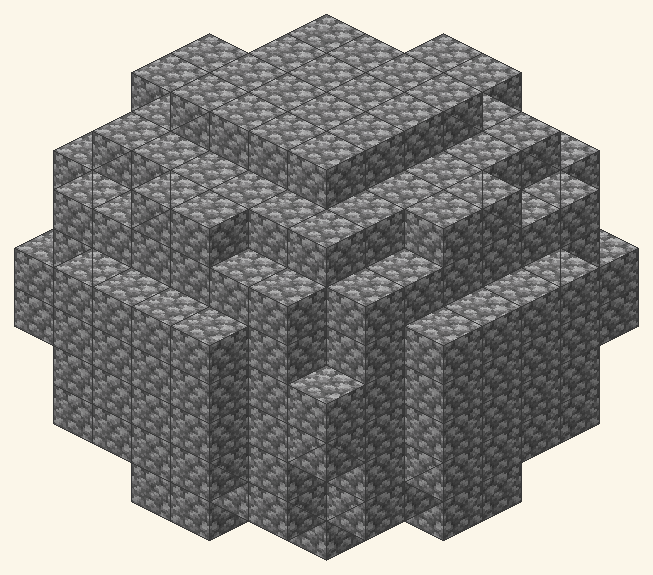
\includegraphics[width=0.55\linewidth]{fig10_3d_sphere_d12.png}\\[0.4em]
    {\sffamily\footnotesize\color{muted}Сфера диаметра 10, воксели\-зированная при помощи Block Round и визуализированная с текстурой \emph{cobblestone} (булыжник) из Minecraft.}
  \end{minipage}
  \vspace{0.7cm}\\
  {\color{rule}\rule{0.6\textwidth}{0.6pt}\par}
  \vspace{0.9cm}
  \begin{minipage}{0.82\textwidth}
    \centering\sffamily\small\color{muted}
    \textbf{Интегрируемые области:} Математика $\cdot$ Информатика $\cdot$ Цифровое искусство и дизайн $\cdot$ Цифровая грамотность $\cdot$ Образование через игру \\[0.4em]
    \textbf{Соответствие нормативной базе:} ФГОС СОО (приказ Минпросвещения от 12.08.2022 № 732) $\cdot$ Базовый и углублённый уровни математики $\cdot$ ЕГЭ $\cdot$ \hyperref[sec:olimp]{ВсОШ} $\cdot$ национальный проект «Образование»
  \end{minipage}
\end{titlepage}

% =============================================================================
\renewcommand{\contentsname}{\color{accent}Содержание}
\tableofcontents
\thispagestyle{fancy}
\newpage

% =============================================================================
\section{Идентификация и контекст}\label{sec:identificacao}

\begin{center}
\begin{tabular}{@{}p{0.32\textwidth}p{0.62\textwidth}@{}}
\toprule
\textbf{Учебный предмет} & Математика (с глубокой межпредметной интеграцией: информатика, изобразительное искусство, инженерия, история, география). \\
\addlinespace[2pt]
\textbf{Уровень и класс} & Среднее общее образование --- 11-й класс (выпускной класс). Адаптируется для 10-го класса и для вечерней (сменной) школы. \\
\addlinespace[2pt]
\textbf{Охватываемые формы обучения} & Общеобразовательная школа, лицей, гимназия, школы с углублённым изучением математики/информатики (СУНЦ МГУ имени Колмогорова, СУНЦ НГУ, СУНЦ СПбГУ, СУНЦ УрФУ), вечерняя школа, заочная форма, центры «Точка роста» в сельских школах, технопарки «Кванториум». \\
\addlinespace[2pt]
\textbf{Учебная нагрузка} & 5 уроков по 50 минут (250 мин аудиторной работы) + опциональная внеурочная деятельность. Вариант из 2 спаренных пар по 100 минут описан в §\ref{sec:adapt}. \\
\addlinespace[2pt]
\textbf{Основной ресурс} & Block Round --- бесплатное \emph{веб-приложение}, не требует регистрации и сервера, работает офлайн в браузере (PWA). В соответствии с ФЗ-152 «О персональных данных»: не собирает и не передаёт персональных данных. Запускается на недорогом \emph{смартфоне} --- не требует Java и не требует установки Minecraft. \\
\addlinespace[2pt]
\textbf{Разделы ФГОС СОО} & Геометрия и стереометрия (окружность, эллипс, шар, эллипсоид) $\cdot$ Алгебра и начала анализа (объёмы тел вращения, интегральное исчисление) $\cdot$ Цифровая грамотность и проектная деятельность. \\
\addlinespace[2pt]
\textbf{Профили обучения (ФГОС СОО)} & Естественно-научный, технологический, физико-математический (основные); универсальный (адаптируемо). Подходит для проектной и исследовательской деятельности, для индивидуального учебного проекта в 11 классе, для предпрофильной подготовки. \\
\addlinespace[2pt]
\textbf{Олимпиады и внешние связи} & \hyperref[sec:olimp]{ВсОШ по математике} (Всероссийская олимпиада школьников) $\cdot$ ВсОШ по информатике $\cdot$ Турнир городов $\cdot$ ВКОШП $\cdot$ Codeforces $\cdot$ образовательный центр «Сириус» в Сочи. \\
\addlinespace[2pt]
\textbf{Предварительные знания учащихся} & Координатная плоскость; уравнение окружности (10 класс); площадь и объём элементарных фигур; понятие функции; пропорция и проценты. Знакомство с \emph{Minecraft} (желательно, но не обязательно; программа \emph{Block Round} в нём не нуждается). \\
\addlinespace[2pt]
\textbf{Подготовка учителя} & 20 минут предварительного знакомства с Block Round; чтение \texttt{docs\_math/Block\_Round\_Math\_ru-RU.pdf} (технический документ на русском языке); по желанию --- знакомство с командами \cmd{/fill}, \cmd{/clone} и \cmd{//sphere} из Minecraft Java Edition. \\
\bottomrule
\end{tabular}
\end{center}

\begin{zametka}[Разнообразие российской школы]
Эта последовательность разработана с учётом неоднородности российской системы среднего образования: общеобразовательная школа в Москве, Санкт-Петербурге, Новосибирске, Екатеринбурге или Казани; физико-математический лицей или СУНЦ; сельская школа с центром «Точка роста»; школа в национальной республике (Татарстан, Башкортостан, Якутия, Чечня) с двуязычным обучением; школа коренных малочисленных народов Севера, Сибири и Дальнего Востока; вечерняя школа; кадетский корпус или нахимовское/суворовское училище. Каждый из этих контекстов требует особой адаптации, и эти адаптации представлены в §\ref{sec:adapt}. Block Round выбран потому, что \emph{подходит для всех этих сценариев}: запускается на бюджетном смартфоне, не требует постоянного интернета после первичной загрузки (PWA), не нуждается в регистрации и не собирает персональных данных --- условие, прямо вытекающее из ФЗ-152 «О персональных данных» и ФЗ-436 «О защите детей от информации».
\end{zametka}

\begin{minecraft}[Почему именно Minecraft как опорный образ]
Minecraft --- самая продаваемая компьютерная игра в истории (свыше 300 миллионов копий по всему миру). В России это поперечный культурный ориентир для подростков всех регионов и социальных групп; среди российских стримеров и блогеров игры выделяются TheBrainDit, EvgenBro, Frost Bee, Compot, Олег Брейн, FILIPIN, JoY, Diamondrush и многие другие, что подтверждается данными ВЦИОМ и НИУ ВШЭ о медиапотреблении подростков. Любопытно, что задолго до Minecraft именно советский программист Алексей Пажитнов в 1984 году создал в Москве игру «Тетрис» --- по сути, одно из первых массовых произведений воксельного и пиксельного искусства. Таким образом, опора последовательности на Minecraft не дань моде, а признание того, что русский подросток уже живёт внутри геометрии: в традиции, идущей от Тетриса к современным серверам.
\end{minecraft}

% =============================================================================
\section{Педагогическое обоснование}\label{sec:justificativa}

Выбор Block Round в качестве учебного артефакта для 11-го класса отвечает на \acc{пятикратный} запрос современного российского образования: интеграция формальной математики и цифровой грамотности (метапредметные результаты ФГОС СОО); контекстуализация абстрактного знания в практиках, \emph{значимых} для учащегося; подготовка к задачам по стереометрии и функциональным зависимостям, постоянно встречающимся в ЕГЭ (как профильном, так и базовом); реализация принципов национального проекта «Образование» (2018--2030) в части цифровой образовательной среды; и мобилизация культурного мира видеоигры \emph{Minecraft} как мотивационного моста --- без потери математической строгости.

\emph{Воксельное искусство} занимает центральное место в воображении современных российских подростков. \emph{Minecraft} --- игра, появившаяся в 2009 году и приобретённая корпорацией Microsoft в 2014 году за 2{,}5 миллиарда долларов, --- стала самым универсальным культурным ориентиром подросткового поколения. Опора на воксельное строительство превращает привычную \emph{игровую} традицию в \emph{подлинную математическую задачу}: описание аналитически заданных фигур в $\mathbb{R}^3$ на дискретной сетке кубиков $1\times1\times1$. Ученик, ежедневно строящий башни, круглые фермы и купола на серверах российских сообществ (GhostCraft, Crystal-MC, MineFun, Polar Network), обнаруживает, что то, что он делал по интуиции, имеет формальное имя: \emph{воксе\-лизация}, \emph{дискретная растеризация}, \emph{неявное уравнение эллипсоида}.

Эта дидактическая стратегия вступает в диалог с пятью традициями российской и советской педагогики:

\begin{itemize}[leftmargin=1.3em,itemsep=0.2em,topsep=0.3em]
  \item \acc{Л. С. Выготский} (\emph{Мышление и речь}, 1934; культурно-историческая теория). Понятие \emph{зоны ближайшего развития} прямо применимо: ученик уже умеет интуитивно строить сферы в Minecraft --- задача учителя в том, чтобы провести его за руку от этой интуиции к формальному уравнению, действуя в той зоне, где помощь взрослого ещё необходима, но самостоятельная работа уже возможна. Каждое из заданий 1.2, 2.3, 3.2 спроектировано именно как мост через эту зону.

  \item \acc{В. В. Давыдов} и Д. Б. Эльконин (теория развивающего обучения, 1960--1990-е годы). Block Round напрямую соответствует принципам системы Эльконина--Давыдова: от теоретического обобщения (уравнение окружности) --- к содержательной абстракции, а от неё --- к конкретным частным случаям (три алгоритма, разные радиусы, разные текстуры). Деятельностный подход А. Н. Леонтьева реализуется естественным образом: учащийся не получает знание готовым, а добывает его, манипулируя моделью.

  \item \acc{А. С. Макаренко} (коллективистская педагогика; \emph{Педагогическая поэма}, 1933--1935). Работа в парах и тройках (задания 2.5, 3.2, 5.3) воспроизводит макаренковскую идею о том, что личность формируется в коллективе. Сервер Minecraft --- это, по сути, отряд: распределение ролей, ответственность за общее дело, взаимный контроль качества. Реконструкция Шуховской башни классом на школьном сервере была бы прямой реализацией идеи Макаренко в цифровой среде.

  \item \acc{В. А. Сухомлинский} (\emph{Сердце отдаю детям}, 1969; Павлышская школа). Принцип гуманистической педагогики: знание должно быть пережитым, а не вызубренным. Каждый раз, когда ученик \emph{строит} обсуждаемую сферу --- на бумаге, на экране или в Minecraft, --- происходит именно то, чего хотел Сухомлинский: математика становится живым, чувственно переживаемым опытом, а не набором формул, отчуждённых от ребёнка.

  \item \acc{Этноматематика} (У. Д'Амбросио, 1985; русские этноматематики В. Дробышев, А. Степанов). Три алгоритма Block Round (Евклидов, Брезенхэма, Пороговый) можно прочитать как три разные этноматематики для одной и той же задачи; а популярные среди русскоязычной аудитории Minecraft-тьюториалы по строительству круглых форм составляют \emph{четвёртую} вернакулярную этноматематику --- народную, устную, опосредованную игрой, современную, на русском языке.
\end{itemize}

Программное обеспечение выполняет точную эпистемологическую функцию: оно \emph{не заменяет} алгебру, а \emph{материализует} различие между конкурирующими математическими формулировками. Три алгоритма соответствуют трём математически различным определениям одного и того же объекта --- дискретной окружности --- и порождают зримо различающиеся изображения, как показано на рис.~\ref{fig:comp-d10}. Ученик \emph{видит глазами}, что \emph{определение имеет значение}, и одновременно осознаёт, что результат не абстрактен: \emph{он может сложить эту фигуру блок за блоком в Minecraft}.

\begin{figure}[!htbp]
\centering
\begin{subfigure}[t]{0.31\linewidth}\centering
  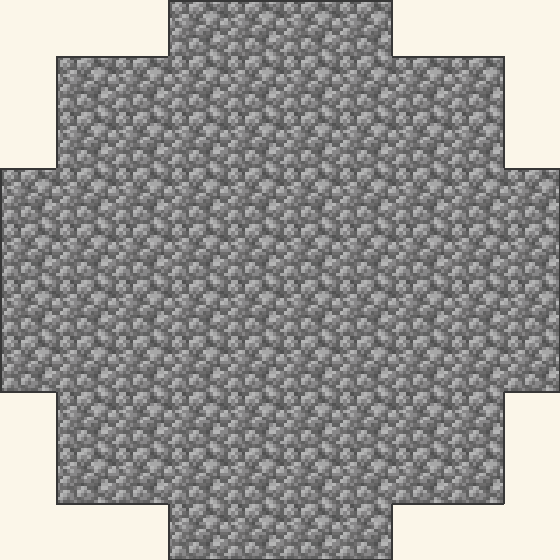
\includegraphics[width=\linewidth]{fig01_2d_d10_euclidean.png}
  \caption{\emph{Евклидов}}
\end{subfigure}\hfill
\begin{subfigure}[t]{0.31\linewidth}\centering
  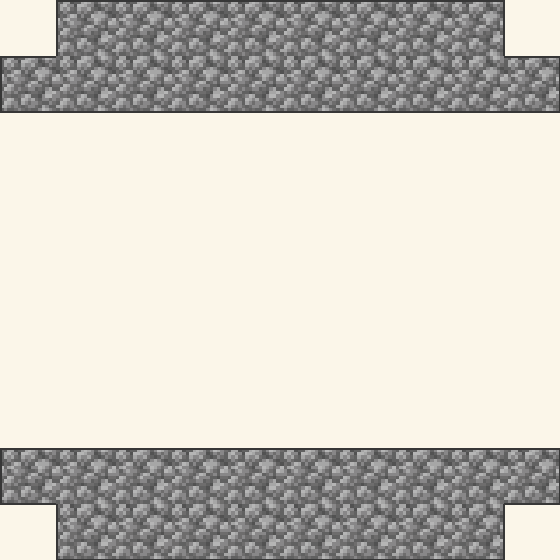
\includegraphics[width=\linewidth]{fig02_2d_d10_bresenham.png}
  \caption{\emph{Брезенхэма}}
\end{subfigure}\hfill
\begin{subfigure}[t]{0.31\linewidth}\centering
  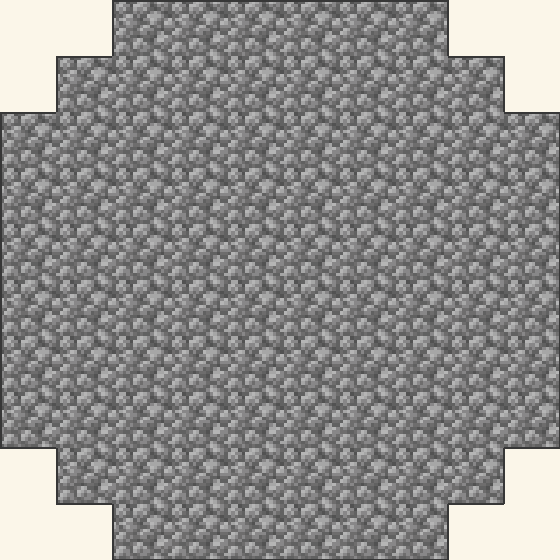
\includegraphics[width=\linewidth]{fig03_2d_d10_threshold.png}
  \caption{\emph{Пороговый}}
\end{subfigure}
\caption{Одна и та же окружность диаметра 10 при трёх критериях принадлежности, отрисованная с текстурой \emph{cobblestone} (булыжник) из Minecraft. Обратите внимание, как угловая клетка, переход между строками и кардинальные точки меняются от рисунка к рисунку --- это три \emph{математически корректных} ответа при разных критериях и три разных плана постройки в \emph{Minecraft}.}
\label{fig:comp-d10}
\end{figure}

\begin{zametka}[Равные возможности и материальная реальность российской школы]
Выбор Block Round частично отвечает на конкретную материальную проблему --- неравенство доступа к цифровым ресурсам между разными школами Российской Федерации. По данным Росстата (ИКТ-индикаторы в образовании, 2023) и НИУ ВШЭ, уровень оснащённости компьютерными классами заметно различается по регионам: от практически 100\,\% в школах Москвы и крупных областных центров до значительно меньших значений в труднодоступных населённых пунктах. С другой стороны, проникновение смартфонов среди подростков 15--17 лет превышает 95\,\% во всех регионах. Block Round создавался именно для такого сценария: бюджетный \emph{смартфон}, отсутствие постоянного интернета, отсутствие регистрации. А когда и этого нет --- Приложение~\ref{ap:adapt-analog} предлагает \emph{полностью бумажный} вариант на клетчатой бумаге. Дополнительный плюс: с 2019 года в сельских школах открывают центры «Точка роста», оборудованные компьютерами и интернетом, --- к моменту 2026 года их более 11\,000 по стране.
\end{zametka}

\begin{minecraft}[Исследования: Minecraft в российском образовании]
Образовательный потенциал Minecraft в России изучается с середины 2010-х годов в публикациях Российской академии образования, в материалах ежегодной конференции «Современные информационные технологии в образовании», в работах НИУ ВШЭ. В частности, в журнале «Информатика в школе» и «Информатика и образование» неоднократно описывались опыты применения Minecraft на уроках информатики и математики. В каталоге сервисов Сферум, Учи.ру, РЭШ (Российская электронная школа) присутствуют ссылки на игровые сценарии. С 2022 года Minecraft Education Edition в России частично ограничен в распространении, однако \emph{Java Edition} остаётся доступной по официальной лицензии Mojang/Microsoft; российские серверы продолжают работать. \emph{Block Round служит мостом}: он работает без установки Minecraft, без аккаунта и без подключения к зарубежным сервисам, что соответствует требованию импортонезависимости, артикулированному Минпросвещения России для образовательных продуктов.
\end{minecraft}

% =============================================================================
\section{Цели обучения}\label{sec:objetivos}

\subsection{Общая цель}

Привести учащихся к \acc{пониманию, сравнению, использованию и переводу-в-постройку} формальных определений окружности, эллипса и эллипсоида как критериев включения клеток в дискретную сетку текстурированных вокселей; мобилизовать неявное уравнение этих фигур для объяснения, прогнозирования, модификации и \emph{строительства в Minecraft} авторских визуальных композиций, в диалоге с визуальным наследием русского авангарда (Малевич, Лисицкий, Татлин), русского деревянного зодчества (Кижи), традиционным жильём коренных народов России (чум, яранга, юрта) и с математической традицией России. Понимание множественности правильных ответов вписывает работу в \emph{русскую математическую традицию} --- одну из сильнейших в мире, давшую десять обладателей Филдсовской медали (от С. П. Новикова в 1970 году до С. К. Смирнова в 2010), включая Г. Я. Перельмана, отказавшегося от премии после доказательства гипотезы Пуанкаре в 2003 году, и в традицию русскоязычного Minecraft-сообщества, где сообщества давно строят города из круглых форм, не давая им формального математического имени.

\subsection{Конкретные задачи}

\textbf{Когнитивные (понятийные):}
\begin{itemize}[leftmargin=1.3em,itemsep=0.2em,topsep=0.3em]
  \item опознавать неявное уравнение $\left(\dfrac{x}{r_x}\right)^{\!2} + \left(\dfrac{y}{r_y}\right)^{\!2} = 1$ как общий случай, включающий окружность $x^2 + y^2 = r^2$;
  \item понимать, что три различных критерия принадлежности (расстояние от центра, серединная точка Брезенхэма, покрытие угла клетки) дают три разных множества клеток --- как показано на рис.~\ref{fig:comp-d10};
  \item осваивать переход от уравнения 2D к уравнению 3D эллипсоида и связывать его с формулой объёма $V = \tfrac{4}{3}\pi r_x r_y r_z$ (тема, регулярно встречающаяся на ЕГЭ профильного уровня в задачах по стереометрии);
  \item интерпретировать сечение тела плоскостью как \emph{линейное неравенство}, применённое к координатам вокселей;
  \item понимать \emph{арифметику инвентаря Minecraft} (стаки по 64 предмета, обычные сундуки на 27 ячеек, двойные сундуки на 54 ячейки) как конкретное приложение \emph{деления с округлением вверх} и \emph{представления частного и остатка};
  \item опознавать \emph{симметрии} (отражение, поворот), позволяющие построить целую сферу из одного октанта с помощью команды \cmd{/clone}.
\end{itemize}

\textbf{Процедурные:}
\begin{itemize}[leftmargin=1.3em,itemsep=0.2em,topsep=0.3em]
  \item оперировать интерфейсом Block Round в обоих режимах (2D и 3D) и экспортировать изображения в формате PNG и схемы в формате \texttt{.schem};
  \item строить от руки, на клетчатой бумаге, дискретное приближение окружности по евклидову критерию и проверять его в программе;
  \item вычислять дискретную площадь/объём воксе\-лизированной фигуры подсчётом клеток и сравнивать с непрерывными значениями, выражая результат в виде относительной погрешности;
  \item составлять авторскую фигуру, комбинируя окружности, эллипсы и эллипсоиды с математически обоснованным выбором, прогнозируя количество блоков каждого типа и количество необходимых двойных сундуков;
  \item импортировать экспортированную из Block Round схему в Litematica или Schematica (моды для Minecraft) и реализовывать постройку в игре;
  \item записывать последовательность команд \cmd{/clone}, превращающую один октант в полную сферу.
\end{itemize}

\textbf{Поведенческие (ценностные):}
\begin{itemize}[leftmargin=1.3em,itemsep=0.2em,topsep=0.3em]
  \item сотрудничать в парах или тройках при выполнении практических заданий, моделируя работу команды строителей сервера Minecraft;
  \item математически аргументировать эстетический выбор --- умение, прямо необходимое в задании повышенной сложности профильного ЕГЭ по математике и в защите индивидуального учебного проекта в 11-м классе;
  \item принимать, что у реальной задачи (например, «построить купол из Quartz на сервере класса») может быть несколько технически корректных решений;
  \item выявлять математические образцы в культурном наследии России (русский авангард, традиционная архитектура), в традиционных знаниях коренных народов и в современной цифровой культуре (российские стримеры, серверы Minecraft);
  \item развивать \emph{цифровую этику}: уважать работу одноклассников, указывать источники переиспользованных построек, понимать смысл лицензии.
\end{itemize}

% =============================================================================
\section{Соответствие ФГОС СОО}\label{sec:fgos}

Дидактическая последовательность опирается напрямую на \acc{четыре блока} планируемых результатов раздела «Математика» в Федеральном государственном образовательном стандарте среднего общего образования (ФГОС СОО, приказ Минобрнауки от 17.05.2012 № 413 в редакции приказа Минпросвещения от 12.08.2022 № 732). Она же связана с метапредметным блоком «Цифровая грамотность и проектная деятельность», а также с предметами «Информатика», «Изобразительное искусство» и «История».

\begin{standart}[Геометрия и стереометрия]
Применять \acc{разные методы} для нахождения площади поверхности и объёма геометрических тел (шар, цилиндр, конус, эллипсоид) методом разбиения и аппроксимации, \acc{выводить} формулы и применять их в реальных ситуациях, \emph{в том числе с использованием цифровых технологий}. Сравнивать непрерывные значения с дискретными приближениями.
\end{standart}

\begin{standart}[Алгебра и начала анализа]
Решать задачи на вычисление \acc{объёмов и площадей} тел вращения, применяя интегральное исчисление, понимать связь интеграла Римана и предельной суммы дискретных приближений. Использовать понятие функции, её областей определения и значений, монотонности.
\end{standart}

\begin{standart}[Аналитическая геометрия плоскости и пространства]
Записывать и применять уравнения окружности, эллипса, шара и эллипсоида (как геометрических мест точек). Применять координатный метод для решения задач на расстояния, симметрии и сечения.
\end{standart}

\begin{standart}[Цифровая грамотность и проектная деятельность]
Применять цифровые инструменты для исследования математических объектов, оформлять и защищать индивидуальный учебный проект в 11 классе, \acc{переводить} модель из алгебраической формы в графическую и в воксельную форму, обосновывать выбор инструмента.
\end{standart}

\medskip
Также мобилизуются \emph{метапредметные результаты} ФГОС СОО:

\begin{itemize}[leftmargin=1.3em,itemsep=0.15em,topsep=0.3em]
  \item \acc{Метапредметный блок 3} --- умение строить модели для решения задач, оценивать правдоподобность результатов и анализировать погрешности;
  \item \acc{Метапредметный блок 4} --- гибкое использование разных форм представления (алгебраической, геометрической, компьютерной, воксельной);
  \item \acc{Метапредметный блок 5} --- исследовательская и проектная деятельность, формулирование гипотез и их проверка с использованием цифровых технологий.
\end{itemize}

\subsection{Соответствие требованиям ЕГЭ}\label{sec:ege}

Представленные ожидаемые результаты прямо соотносятся со следующими элементами кодификатора ЕГЭ по математике (профильный уровень):

\begin{itemize}[leftmargin=1.3em,itemsep=0.15em,topsep=0.3em]
  \item Раздел \emph{Геометрия}: объём шара, цилиндра, конуса, пирамиды; площади поверхностей; задачи 8 и 14 профильного ЕГЭ традиционно посвящены стереометрии и тесно связаны со сферической геометрией;
  \item Раздел \emph{Алгебра и начала анализа}: задачи на функции, графики, исследование функций; задача 12 профильного ЕГЭ часто требует исследования и построения графика;
  \item Раздел \emph{Уравнения и неравенства}: системы неравенств, линейные неравенства как условия принадлежности областей плоскости и пространства.
\end{itemize}

Также материал прямо связан с заданиями ЕГЭ по информатике: задачи на двоичную арифметику, представление информации, алгоритмическое мышление --- особенно задачи 11, 16 и 25 актуального кодификатора. Демоверсии ЕГЭ публикуются на портале ФИПИ (\url{https://fipi.ru}).

\subsection{Цифровая грамотность и общероссийский контекст}

Тема \acc{Цифровая грамотность} пронизывает всю последовательность. Обсуждаются вопросы \emph{цифровой этики} (лицензии свободного и проприетарного программного обеспечения; Block Round распространяется как открытое программное обеспечение в браузере), \emph{защиты персональных данных} (\href{http://www.consultant.ru/document/cons_doc_LAW_61801/}{Федеральный закон от 27.07.2006 № 152-ФЗ «О персональных данных»}; ФЗ-149 «Об информации, информационных технологиях и о защите информации»; ФЗ-436 «О защите детей от информации»), \emph{авторских прав} (творческие работы учащихся в Уроке~\ref{aula5}) и \emph{цифрового гражданства} (ответственное поведение на серверах Minecraft, противодействие гриферству и буллингу в сети).

% =============================================================================
\section{Содержание обучения}\label{sec:conteudos}

\subsection{Понятийное содержание}
\begin{itemize}[leftmargin=1.3em,itemsep=0.15em,topsep=0.3em]
  \item Декартова система координат в $\mathbb{R}^2$ и $\mathbb{R}^3$; центр клетки \emph{против} угла клетки.
  \item Каноническое уравнение окружности: $x^2 + y^2 = r^2$.
  \item Общее неявное уравнение эллипса: $\left(\dfrac{x}{r_x}\right)^{\!2} + \left(\dfrac{y}{r_y}\right)^{\!2} = 1$.
  \item Неравенство принадлежности: \emph{внутренность, внешность} и \emph{граница}.
  \item Уравнения эллипсоида и сферы в $\mathbb{R}^3$.
  \item Непрерывный объём эллипсоида: $V = \tfrac{4}{3}\pi r_x r_y r_z$.
  \item Плоскости в пространстве как линейные неравенства (операция сечения).
  \item Окрестность клетки (4-связная в 2D, 6-связная в 3D).
  \item \acc{Арифметика инвентаря Minecraft}: стаки по 64; обычные сундуки (27 ячеек) и двойные сундуки (54 ячейки); деление с округлением вверх $N_{\mathrm{packs}} = \lceil N/64 \rceil$.
  \item \acc{Октаэдрическая симметрия} и группа $\mathbb{Z}_2^3$ координатных отражений (подгруппа порядка 8 группы $O_h$): применение в оптимизированном строительстве с помощью \cmd{/clone}.
\end{itemize}

\subsection{Процедурное содержание}
\begin{itemize}[leftmargin=1.3em,itemsep=0.15em,topsep=0.3em]
  \item Ручное построение на клетчатой бумаге по явному критерию.
  \item Работа с Block Round (смена режима, регулировка \emph{слайдеров}, выбор алгоритма, экспорт в PNG и \texttt{.schem}).
  \item Сравнение дискретных и непрерывных площадей/объёмов подсчётом клеток.
  \item Композиция комбинированных фигур (авторское \emph{воксельное искусство} с геометрическим обоснованием).
  \item Импорт \texttt{.schem} в Litematica/Schematica.
  \item Выполнение ванильных команд \cmd{/fill}, \cmd{/clone}, \cmd{/setblock} и команд WorldEdit \cmd{//sphere}, \cmd{//hsphere}, \cmd{//ellipsoid}.
  \item Планирование добычи материала в режиме выживания.
\end{itemize}

\subsection{Ценностное содержание}
\begin{itemize}[leftmargin=1.3em,itemsep=0.15em,topsep=0.3em]
  \item Сотрудничество в парах и тройках.
  \item Аргументированная защита решений (математическое обоснование выбора).
  \item Цифровая этика: уважение к лицензии программы, к работе одноклассников и к правилам общего сервера Minecraft.
  \item Признание ценности математических образцов в русском культурном наследии и в современной цифровой культуре.
\end{itemize}

\subsection{Режимы визуализации и разнообразие алгоритмов}

Помимо смены алгоритма, Block Round предоставляет три \emph{режима визуализации} (Заполненный, Тонкий, Толстый), порождающих разные изображения одной и той же геометрической фигуры, как видно на рис.~\ref{fig:render-modes}. В Minecraft этим режимам соответствуют три типа построек: \emph{Заполненная} сфера использует все блоки внутри (массивный купол из Stone); \emph{Тонкая} оставляет только оболочку (полый купол для зала или музея); \emph{Толстая} закрывает диагональные щели, остающиеся в режиме Тонкий, --- \emph{это необходимо} для куполов из стекла или льда под водой, которые должны быть герметичны.

\begin{figure}[!htbp]
\centering
\begin{subfigure}[t]{0.31\linewidth}\centering
  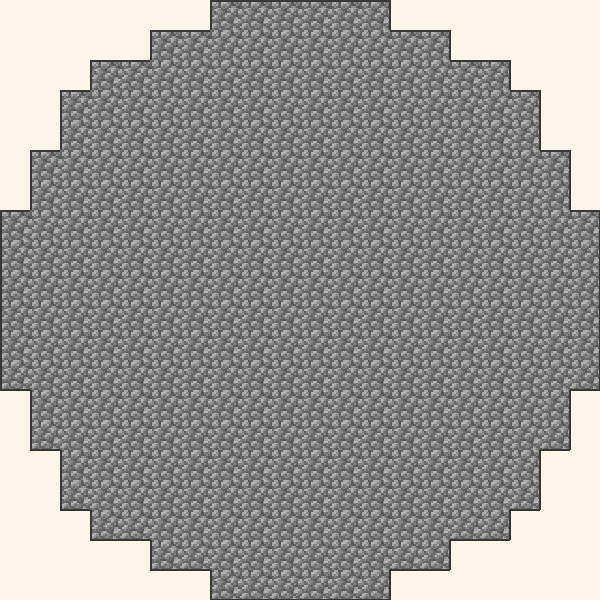
\includegraphics[width=\linewidth]{fig04_2d_d20_euclidean.png}
  \caption{\emph{Заполненный}}
\end{subfigure}\hfill
\begin{subfigure}[t]{0.31\linewidth}\centering
  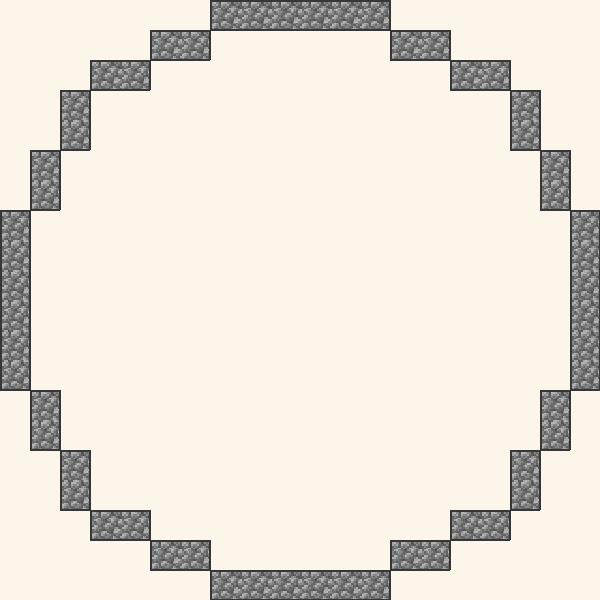
\includegraphics[width=\linewidth]{fig08_2d_d20_thin.png}
  \caption{\emph{Тонкий} (контур в 1 блок)}
\end{subfigure}\hfill
\begin{subfigure}[t]{0.31\linewidth}\centering
  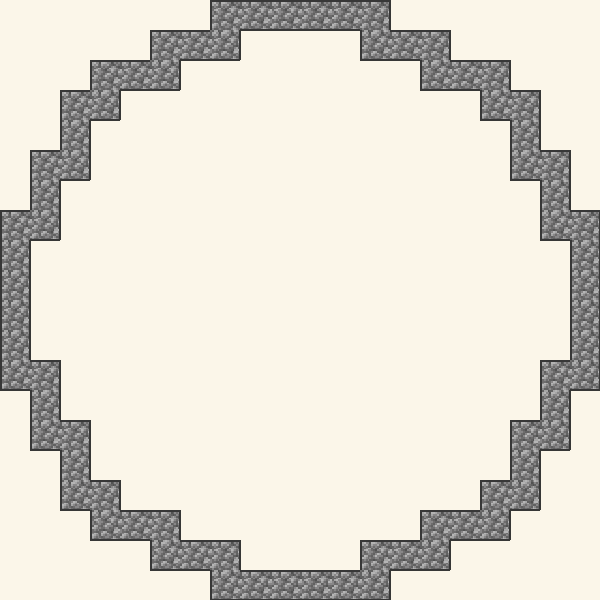
\includegraphics[width=\linewidth]{fig09_2d_d20_thick.png}
  \caption{\emph{Толстый} (контур с диагональными мостами)}
\end{subfigure}
\caption{Три режима визуализации для одной и той же евклидовой окружности диаметра 20. Режим \emph{Тонкий} соответствует топологической дискретной границе; режим \emph{Толстый} добавляет блоки по диагоналям, чтобы избежать дырок в углах $45^\circ$ --- именно эта проблема возникает в куполе из стекла под водой в Minecraft, где диагональная щель пропускает воду.}
\label{fig:render-modes}
\end{figure}

\subsection{Текстуры блоков: отличительная черта Block Round}

Хотя математика \emph{отбора вокселей} не зависит от текстуры, Block Round визуализирует каждый воксель его канонической шестиугольной текстурой из Minecraft. Одна и та же сфера диаметра 10 полностью меняет визуальный характер в зависимости от выбранного блока (рис.~\ref{fig:textures}), \emph{без всяких изменений в основном алгоритме}. В этом главный педагогический смысл: \emph{форма} есть плод математики, \emph{внешний вид} --- последующее эстетическое решение.

\begin{figure}[!htbp]
\centering
\begin{subfigure}[t]{0.31\linewidth}\centering
  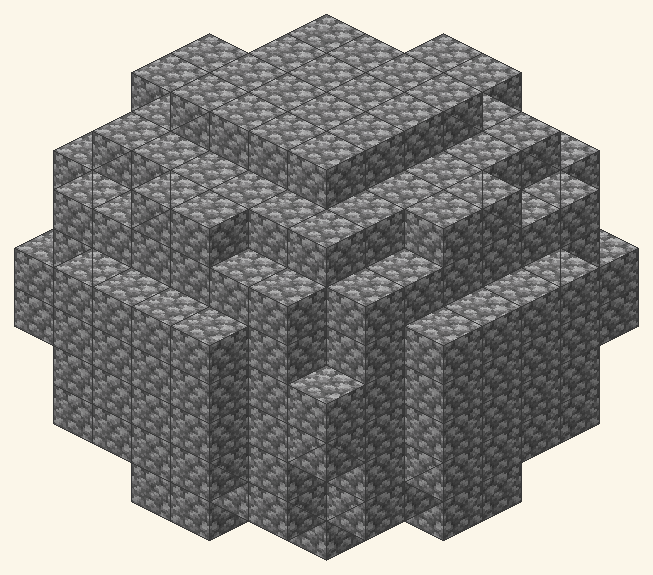
\includegraphics[width=\linewidth]{fig15_3d_sphere_cobblestone.png}
  \caption{\emph{Cobblestone}}
\end{subfigure}\hfill
\begin{subfigure}[t]{0.31\linewidth}\centering
  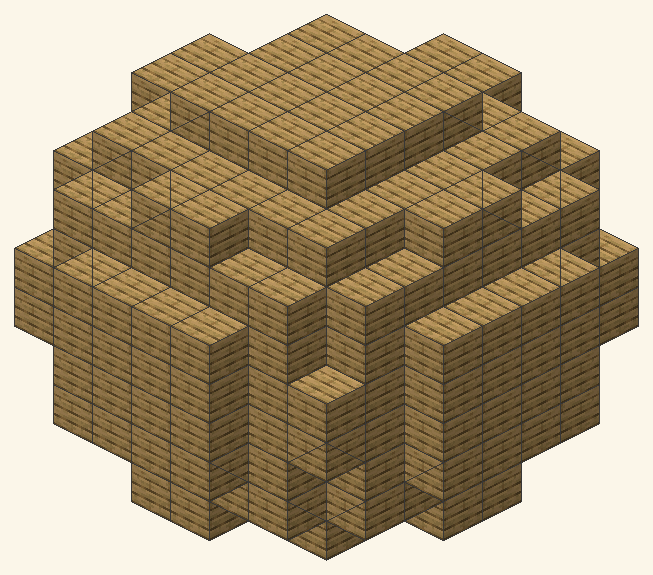
\includegraphics[width=\linewidth]{fig17_3d_sphere_oak.png}
  \caption{\emph{Oak Planks}}
\end{subfigure}\hfill
\begin{subfigure}[t]{0.31\linewidth}\centering
  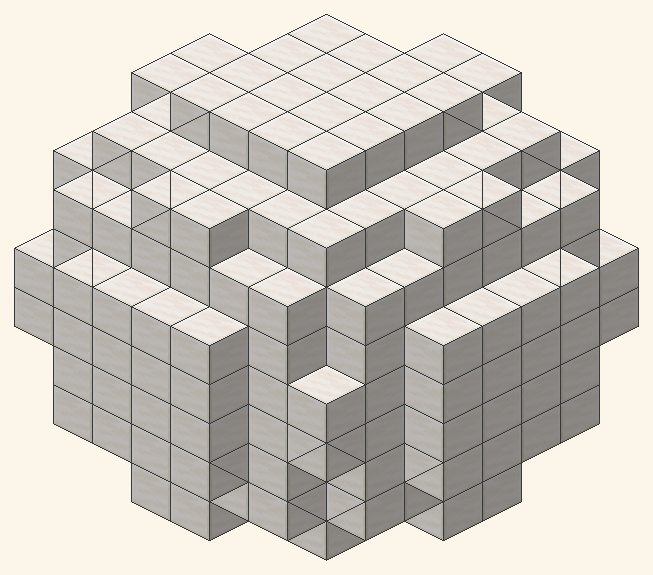
\includegraphics[width=\linewidth]{fig19_3d_sphere_quartz.png}
  \caption{\emph{Quartz Block}}
\end{subfigure}
\caption{Три текстуры Minecraft, применённые к \emph{одной} сфере диаметра 10. Воксельный силуэт у всех трёх версий идентичен --- математика не изменилась. Что меняется, так это визуальный характер: \emph{Cobblestone} напоминает средневековую стену, \emph{Oak Planks} --- интерьер деревянной избы или корабля, \emph{Quartz Block} --- современный храм или белокаменную церковь.}
\label{fig:textures}
\end{figure}

% =============================================================================
\section{Предварительные знания}\label{sec:prerrequisitos}

Последовательность предполагает предшествующее знакомство со следующим материалом:

\begin{itemize}[leftmargin=1.3em,itemsep=0.15em,topsep=0.3em]
  \item Декартова система координат: положение точек $(x, y)$ и $(x, y, z)$.
  \item Каноническое уравнение окружности (содержание 10 класса).
  \item Площади многоугольников и круга; объёмы куба, призмы и цилиндра (10--11 класс, стереометрия).
  \item Понятие функции: область определения, область значений, график.
  \item Пропорция и проценты.
  \item Целочисленное деление с частным и остатком (5--6 класс, основная школа).
\end{itemize}

\emph{Факультативное предварительное знание (не обязательное, но полезное):} знакомство с Minecraft. Эта последовательность сознательно построена так, чтобы её могли пройти даже учащиеся, которые \emph{никогда} не играли в Minecraft (редкая, но возможная ситуация, особенно в сельских школах с ограниченным интернетом) --- вся работа идёт в Block Round, самодостаточном в браузере.

Если у класса обнаруживаются пробелы в одном из обязательных пунктов выше --- частая реальность для постпандемийного периода 2020--2022 годов, отражённая в исследованиях НИУ ВШЭ и в данных Рособрнадзора по результатам ВПР (Всероссийские проверочные работы), --- то Урок~1 предусматривает 10-минутный \emph{диагностический модуль}, описанный в §\ref{aula1}.

% =============================================================================
\section{Ресурсы и материалы}\label{sec:recursos}

\subsection{Цифровые ресурсы}
\begin{itemize}[leftmargin=1.3em,itemsep=0.15em,topsep=0.3em]
  \item Block Round (один экземпляр на учащегося \emph{или} на пару);
  \item Проектор, телевизор с HDMI-входом или интерактивная доска;
  \item Доступ в \emph{компьютерный класс}, \emph{или} использование личных \emph{смартфонов} учащихся (модель BYOD --- \emph{Bring Your Own Device}), \emph{или} \emph{планшеты}, выдаваемые школой (в Москве --- по программе МЭШ);
  \item (Опционально, Урок~\ref{aula5}) доступ к Minecraft Java Edition с установленными модами \emph{Litematica} или \emph{Schematica}; альтернативно --- использование ванильной версии с командами \cmd{/fill} и \cmd{/clone}.
\end{itemize}

\subsection{Аналоговые ресурсы}
\begin{itemize}[leftmargin=1.3em,itemsep=0.15em,topsep=0.3em]
  \item Клетчатая бумага (1\,см), 2 листа на ученика;
  \item Простой карандаш, ластик, линейка 30\,см;
  \item Цветные карандаши или фломастеры (предпочтительно травянисто-зелёный \texttt{\#5B8E3F} и земляно-коричневый \texttt{\#825432} --- палитра Block Round);
  \item Лист с упражнениями (Приложение~\ref{ap:exerc});
  \item Меловая или маркерная доска.
\end{itemize}

\subsection{Учебники и федеральный перечень}\label{sec:fpu}

Block Round дополняет --- но не заменяет --- учебник математики, выбранный школой из \href{https://fpu.edu.ru/}{Федерального перечня учебников} (ФПУ). Издания, особенно хорошо сочетающиеся с темами последовательности:

\begin{itemize}[leftmargin=1.3em,itemsep=0.1em,topsep=0.2em,nosep]
  \item \emph{Геометрия. 10--11 классы} --- Л. С. Атанасян, В. Ф. Бутузов и др. (Просвещение);
  \item \emph{Алгебра и начала математического анализа. 10--11 классы} --- А. Г. Мордкович (Мнемозина);
  \item \emph{Геометрия. 10--11 классы} --- А. В. Погорелов (Просвещение);
  \item \emph{Алгебра и начала анализа. 10--11 классы} --- Ю. М. Колягин, М. В. Ткачёва, Н. Е. Фёдорова (Просвещение);
  \item \emph{Геометрия. 10--11 классы. Углублённый уровень} --- А. Д. Александров, А. Л. Вернер, В. И. Рыжик (Просвещение).
\end{itemize}

Главы об \emph{уравнении окружности}, о \emph{кониках} и о \emph{стереометрии метрических вычислений} (объёмы) прямо связаны с последовательностью. В частности, задачи на \emph{покрытие}, \emph{мощение} и \emph{подсчёт на сетках} (часты в учебниках Атанасяна и Мордковича) почти тождественны центральной задаче Block Round --- лишь с другой терминологией.

\subsection{Доступ к Block Round}

В порядке предпочтительности:

\begin{enumerate}[leftmargin=1.5em,itemsep=0.15em,topsep=0.3em]
  \item \textbf{Хостинг учителя} на \emph{GitHub Pages} или на школьном портале (URL раздаётся через QR-код, проецируемый на доску). Публичная версия: \url{https://vinisouza128.github.io/block-round/}.
  \item \textbf{Локальная копия} файлов проекта в папке компьютерного класса, запускается через \emph{file://}.
  \item \textbf{Офлайн на \emph{смартфоне}} как PWA: достаточно один раз открыть приложение с интернетом, чтобы браузер установил его в офлайн-режиме.
\end{enumerate}

% =============================================================================
\section{Адаптации к плюрализму российской школы}\label{sec:adapt}

Российская система среднего образования необычайно разнообразна --- от Калининграда до Сахалина, от Заполярья до Северного Кавказа, от элитных лицеев Москвы до однокомплектных сельских школ. Настоящая последовательность спроектирована так, чтобы адаптироваться к этому разнообразию, с конкретными вариантами для каждого из контекстов.

\subsection{Школа в столице или крупном городе}
Типичный сценарий Москвы, Санкт-Петербурга, Новосибирска, Екатеринбурга, Казани, Нижнего Новгорода, Ростова-на-Дону, Краснодара. Как правило, имеется компьютерный класс (с общим доступом), интерактивная доска и стабильный Wi-Fi. В Москве \emph{Московская электронная школа} (МЭШ) предоставляет учителям ПК и планшеты, а также готовые сценарии уроков; в Санкт-Петербурге --- АППО (Академия постдипломного педагогического образования). \emph{Это самая простая для реализации полной последовательности конфигурация.}

\subsection{Школа в районном центре или небольшом городе}
Реальность большинства школ России. Компьютерный класс может работать частично. Рекомендуется \emph{модель BYOD} с личными \emph{смартфонами} учащихся, организованными в пары (один смартфон на пару). Block Round запускается без проблем на устройствах Android начиная с 2018 года. Если \emph{Minecraft} недоступен, Урок~\ref{aula5} может сосредоточиться на гипотетических командах (на бумаге, с описанием эффекта) без потери концептуального содержания. Это \acc{самая распространённая} конфигурация в стране.

\subsection{Физико-математический лицей или гимназия с углублённым изучением}
СУНЦ МГУ имени А. Н. Колмогорова --- наследник «Колмогоровского интерната», основанного в 1963 году самим А. Н. Колмогоровым как одна из первых физматшкол СССР, ныне сильнейшая физматшкола страны. СУНЦ НГУ при Новосибирском государственном университете в Академгородке (тоже основан в 1963), СУНЦ СПбГУ, СУНЦ УрФУ, СУНЦ ВШЭ; лицей «Вторая школа» в Москве; 57-я школа Москвы; 239-й физмат лицей Санкт-Петербурга; гимназия 1543 (Москва); школа имени Е. И. Зельманова в Хабаровске. Очень хорошо оснащённые учреждения. Последовательность естественно встраивается в углублённые программы по математике и информатике. Рекомендуется углубить Урок~\ref{aula2} (алгоритм Брезенхэма) с реализацией на Python в компьютерном классе и Урок~\ref{aula5} --- установкой настоящего сервера Minecraft Java в классе для коллективного строительства. В таких школах материал последовательности может послужить основой индивидуального учебного проекта в 11 классе и заявкой на участие в Всероссийской олимпиаде школьников по математике или информатике.

\subsection{Сельская школа и «Точка роста»}
С 2019 года в рамках национального проекта «Образование» в сельских школах России открываются центры «Точка роста», в которых установлены компьютеры, ноутбуки, 3D-принтеры и обеспечен доступ в интернет. К 2026 году их более 11\,000 по стране. Block Round особенно полезен здесь, поскольку работает в любом современном браузере и не требует мощного оборудования. Для совсем удалённых школ (в Заполярье, в труднодоступной местности Сибири и Дальнего Востока, на островах) предусмотрен полностью аналоговый вариант (Приложение~\ref{ap:adapt-analog}). Урок~\ref{aula3} можно обогатить, опираясь на уже имеющиеся у сельских учеников знания о геометрии --- планировка огородов, теплиц, силосов, круглых загонов для скота. Их традиционное практическое знание становится мостом к формальному уравнению.

\subsection{Школы коренных народов Севера, Сибири и Дальнего Востока}
В соответствии со статьёй 26 Конституции Российской Федерации и \href{http://www.consultant.ru/document/cons_doc_LAW_15524/}{Федеральным законом «О языках народов Российской Федерации»} (1991), в школах с обучением на родном языке коренных народов России --- ненцы Ямало-Ненецкого АО, ханты и манси ХМАО, чукчи Чукотки, эвенки и якуты Республики Саха (Якутия), нивхи Сахалина, нанайцы Хабаровского края, шорцы Кемеровской области и многие другие --- последовательность может быть \emph{обогащена местным знанием}: \emph{чум} ненцев (конический каркас на оленьих шкурах --- геометрия конуса!), \emph{яранга} чукчей и ительменов Камчатки (полусферический каркас!), \emph{юрта} алтайцев, бурятов, якутов (круглая планировка). \emph{Старшие представители общины и учитель родного языка --- незаменимые партнёры в этой адаптации} (см. Урок~\ref{aula3}, Задание~\ref{at:34}). Геометрия традиционного жилища --- это та же геометрия сферы и эллипсоида, что и в учебнике, только материал другой: вместо блоков Quartz --- оленья шкура или войлок.

\subsection{Школы в национальных республиках}
В Республике Татарстан, Башкортостане, Якутии, Чечне, Дагестане, Калмыкии, Бурятии, Туве, Карелии, Удмуртии, Чувашии, Марий Эл и других республиках --- двуязычное обучение (русский язык и государственный язык республики). Учитель может выпустить раздаточные материалы на двух языках; в Казани (Татарстан) интересны проекции на сложную геометрию мечетей (полусферические купола Кул-Шариф) и православных соборов (Благовещенский собор Кремля). В Бурятии и Калмыкии --- буддийские ступы (структура полусферы) и мандалы (круговые орнаменты). В Туве --- горловое пение и геометрия национальных орнаментов кадак. В Якутии --- летние юрты ураса и солярная символика. В Чечне --- башенная архитектура горцев. Всё это --- материал для глубокого диалога между формальной математикой и живой культурой региона.

\subsection{Кадетские корпуса, суворовские и нахимовские училища}
В системе военно-патриотического воспитания (Министерство обороны, МЧС, МВД) есть особый запрос на инженерную и прикладную математику. Последовательность отвечает на этот запрос: симметрия, оптимизация числа блоков, командное распределение задач (Урок~\ref{aula4} --- арифметика инвентаря --- идеально для логистической подготовки), реконструкция исторических крепостей (Брестская крепость, Кремль) на школьном сервере Minecraft. В казачьих школах (Дон, Кубань, Терек, Урал, Забайкалье) можно опираться на казачью архитектуру: курени, станицы, церкви.

\subsection{Вечерняя (сменная) школа и заочная форма}
Обычно вечерние группы: взрослые учащиеся, возвращающиеся к школьному образованию. Block Round хорошо подходит здесь, потому что интерфейс дружественен, а тема (Minecraft, видеоигры) знакома и взрослым: многие из них росли в 2010-е годы и помнят раннюю популярность игры в России. Рекомендуется сократить время каждой активности на 20\,\% (с учётом более короткой вечерней смены) и отдать приоритет устным обсуждениям, а не объёмному письму. Урок~\ref{aula5} может стать \emph{факультативным} для вечерней школы, с фокусом на Уроках 1--4.

\subsection{Вариант 2 спаренных занятий по 100 минут}
Для школ с режимом «пара» (часто в технологических лицеях и СУНЦ): Уроки 1+2 на одной паре, 3+4 на другой, Урок 5 отдельно (на одной паре или на двух при наличии времени для реальной постройки). Итого: 3 пары по 100 минут + 1 пара 50 минут, либо 2 пары по 100 минут + одна пара 200 минут для итоговой практической работы в Minecraft.

\subsection{Сопоставление с региональными программами}

Каждый регион детализирует ФГОС СОО в собственной образовательной программе. Основные центры:

\begin{center}
\small
\begin{tabularx}{\textwidth}{@{}p{0.18\textwidth}p{0.25\textwidth}X@{}}
\toprule
\textbf{Регион} & \textbf{Реферативная программа} & \textbf{Особенности изучения геометрии и стереометрии в 10--11 классе} \\
\midrule
Москва & МЦКО + МЭШ (Московская электронная школа) & Сильный акцент на цифровых инструментах; усиленная стереометрия с использованием GeoGebra и веб-приложений. \\
\addlinespace[3pt]
Санкт-Петербург & СПб АППО + РГПУ им. А. И. Герцена & Классическая школа Кисёлёва / Александрова; работа с углублёнными программами. \\
\addlinespace[3pt]
Республика Татарстан & МОиН РТ; двуязычные программы (русский + татарский) & Углублённая программа КФУ; СУНЦ при КФУ; особое внимание к олимпиадному движению. \\
\addlinespace[3pt]
Республика Саха (Якутия) & МО РС(Я); программы на якутском и русском & Длинные дистанции, особое внимание к дистанционному обучению; «Якутская школа республики» как сеть инновационных школ. \\
\addlinespace[3pt]
Краснодарский край & МОНКК; казачьи кадетские корпуса & Сильная практическая ориентация; интеграция с летними школами в Сочи (центр «Сириус»). \\
\addlinespace[3pt]
Новосибирская область & ИНИПКРО Новосибирск; СУНЦ НГУ & Академгородок: тесная связь с РАН; математические бои; летние школы при НГУ. \\
\addlinespace[3pt]
Чеченская Республика & МОН ЧР; программы на русском и чеченском & Восстановление образовательной системы после 2000-х; интенсивное цифровое оснащение в рамках «Цифровой экономики». \\
\bottomrule
\end{tabularx}
\end{center}

\subsection{Гибридное и дистанционное обучение}
Веб-природа Block Round делает его тривиально совместимым с дистанционными уроками (\emph{Сферум} --- платформа Министерства просвещения; \emph{Учи.ру}; \emph{ЯКласс}; \emph{Российская электронная школа} РЭШ; \emph{МЭШ} в Москве; \emph{Дневник.ру}). Учитель демонстрирует свой экран; учащиеся работают параллельно на своих устройствах. Работу на клетчатой бумаге можно сфотографировать и отправить как асинхронное задание через \emph{ВКонтакте} (группа класса), Сферум, \emph{Дневник.ру} или другую платформу региональной электронной школы. Урок~\ref{aula5} можно провести на общем сервере Minecraft --- \emph{Realms} от Microsoft или собственный сервер на хостинге, --- где класс встречается в виртуальном мире и совместно строит общий проект.

% =============================================================================
\section{Дидактическая последовательность}\label{sec:sequencia}

Последовательность следует структуре \acc{мотивация --- проблематизация --- систематизация --- синтез}, опирающейся на деятельностный подход А. Н. Леонтьева и на теорию развивающего обучения В. В. Давыдова и Д. Б. Эльконина. Каждый урок по 50 минут учитывает когнитивный ритм подростка, чередуя короткие лекционные моменты ($\leq 15$\,мин) с практическими активностями.

% =============================================================================
\subsection{Урок 1 --- «Как игра рисует сферу с помощью кубов?»}\label{aula1}

\subsubsection*{Цель урока}
Сформулировать \emph{центральную проблему} дискретной растеризации как подлинную математическую задачу, мобилизовать уравнение окружности и представить Block Round. Признать, что центральная проблема урока --- \emph{как решить, какие блоки красить?} --- это в точности та проблема, с которой сталкивается каждый игрок Minecraft, строящий сферу в игре.

\begin{zadanie}[1.1 --- Мотивация \quad\tempo{10 мин}]
\textbf{Стратегия:} \emph{think--pair--share} (подумать индивидуально, обсудить в паре, поделиться с классом). \\[0.4em]
\textbf{Шаги:}
\begin{enumerate}[leftmargin=1.5em,itemsep=0.2em,topsep=0.3em,nosep]
  \item Спроецировать (или нарисовать) три классические постройки из Minecraft: стеклянный купол на каменном основании (любой русскоязычный туториал на YouTube --- например, ролики TheBrainDit, EvgenBro, Frost Bee); знаменитая \emph{Гигантская сфера}, построенная коллективно на популярном российском сервере (GhostCraft, Crystal-MC, MineFun); пиксель-арт известного российского персонажа в Minecraft (Чебурашка, Винни-Пух Хитрука, Маша из «Маши и Медведя», или герой игры «Атомное сердце» / любимый футболист «Зенита» или ЦСКА).
  \item Спросить класс: \emph{«Посмотрите внимательно. Как игра решает, какие кубы поставить, чтобы получилась сфера? Есть ли у Minecraft встроенный волшебный циркуль?»}
  \item Каждый ученик индивидуально записывает свой ответ (1\,мин) и затем обсуждает его с соседом по парте (2\,мин).
  \item Коллективный сбор: ключевые ответы фиксируются на доске. Подвести к фундаментальному наблюдению: \emph{«Игра может класть только целые кубы --- как же она выбирает?»}
\end{enumerate}
\end{zadanie}

\begin{zadanie}[1.2 --- Проблематизация \quad\tempo{15 мин}]
\textbf{Стратегия:} ручной рисунок, сопоставленный с формальным определением. \\[0.4em]
\textbf{Материалы:} клетчатая бумага, карандаш. \\[0.4em]
\textbf{Шаги:}
\begin{enumerate}[leftmargin=1.5em,itemsep=0.2em,topsep=0.3em,nosep]
  \item Каждый ученик получает половину листа клетчатой бумаги и отмечает центральную точку области $11 \times 11$ клеток.
  \item Команда: \emph{«Закрасьте лучший круг диаметра 10 (радиус 5), какой у вас получится. \emph{Представьте, что каждый квадратик --- это блок булыжника из Minecraft.} У вас 4 минуты.»}
  \item По истечении времени трое-четверо учеников выходят к доске и воспроизводят свой рисунок на нарисованной мелом/маркером сетке.
  \item Управляемое наблюдение: \emph{«Смотрите. У всех получилось одинаково? Почему нет? Кто прав? Если бы каждый из вас строил эту сферу на одном общем сервере класса, какую это создало бы проблему?»}
  \item Подвести к итогу: \emph{единственного} ответа не существует (это подтверждает уже знакомый рис.~\ref{fig:comp-d10}). Каждый ученик неявно использовал свой собственный \acc{критерий} принадлежности клетки.
\end{enumerate}

\textbf{Этно\-мате\-ма\-ти\-чес\-кая заметка:} использовать этот момент, чтобы упомянуть, что \emph{разнообразие ответов --- это и есть предмет этноматематики} (У. Д'Амбросио). В русскоязычной традиции родственная идея проводилась И. Ф. Шарыгиным и И. М. Гельфандом, основавшим в 1964 году Заочную математическую школу при МГУ. \emph{Само русскоязычное Minecraft-сообщество является культурной группой со своей «этноматематикой»}, передающейся через русскоязычные YouTube-туториалы, через моды, написанные российскими разработчиками, и через национальные сервера (TheBrainDit Сервер, Crystal-MC и др.).
\end{zadanie}

\begin{zadanie}[1.3 --- Систематизация \quad\tempo{15 мин}]
\textbf{Стратегия:} диалогическое изложение с опорой на доску. \\[0.4em]
\textbf{Содержание:}

Неявное уравнение окружности, центрированной в начале координат и радиуса $r$:

\begin{formula}
\centering
$\displaystyle x^2 + y^2 \;=\; r^2$
\end{formula}

Точки \emph{внутри} удовлетворяют $x^2 + y^2 < r^2$; точки \emph{снаружи} --- $x^2 + y^2 > r^2$. Уравнение обобщается до эллипса с полуосями $r_x, r_y$:

\begin{formula}
\centering
$\displaystyle \left(\dfrac{x}{r_x}\right)^{\!2} + \left(\dfrac{y}{r_y}\right)^{\!2} \;=\; 1$
\end{formula}

На сетке блоков (вокселей) задача состоит в том, чтобы решить, какие \acc{клетки} принадлежат внутренности. Разные решения дают разные рисунки. Block Round реализует \emph{три} критерия:

\begin{itemize}[leftmargin=1.3em,itemsep=0.15em,topsep=0.3em]
  \item \acc{Евклидов}: находится ли центр $(i + \tfrac{1}{2},\, j + \tfrac{1}{2})$ клетки внутри?
  \item \acc{Брезенхэма}: исторический алгоритм 1965 года, оперирует только целыми числами.
  \item \acc{Пороговый}: попадает ли какой-нибудь \emph{угол} клетки внутрь?
\end{itemize}

\textbf{Демонстрация:} учитель открывает Block Round, выставляет диаметр 10, переключает три алгоритма; класс наблюдает различия. Подчеркнуть: все три фигуры \emph{математически корректны} при разных критериях. Показать, что приложение позволяет менять текстуру блока --- сфера становится из булыжника, дубовых досок, алмаза, светящегося камня; \emph{форма не меняется}. \emph{Это центральная идея Block Round: форма --- математика, текстура --- эстетический выбор.}
\end{zadanie}

\begin{zadanie}[1.4 --- Синтез \quad\tempo{10 мин}]
\textbf{Стратегия:} немедленное индивидуальное применение. \\[0.4em]
\textbf{Команда:} \emph{«Возвращайтесь к бумаге. Перерисуйте круг диаметра 10, \acc{строго} применяя евклидов критерий: закрашивайте клетку тогда и только тогда, когда центр клетки $(i + 0{,}5,\, j + 0{,}5)$ находится на расстоянии не более 5 от центра.»}

В конце сравните рисунок на бумаге с тем, что выдаёт Block Round в евклидовом алгоритме при диаметре 10 --- визуальный эталон даёт рис.~\ref{fig:comp-d10}~(a). \emph{Они должны совпасть.}
\end{zadanie}

\begin{minecraft}[Связь с игрой]
В \emph{Minecraft Java Edition} с установленным модом WorldEdit команда \cmd{//sphere stone 5} строит ровно ту же фигуру, что Block Round выдаёт в алгоритме \emph{Брезенхэма} при диаметре 10. Ученики, играющие на серверах, могут проверить это дома --- постройки идентичны. \emph{Иными словами, то, что мы изучаем на уроке, --- это не дидактическая симуляция Minecraft, а та самая математика, которой игра пользуется под капотом.}
\end{minecraft}

\subsubsection*{Домашнее задание (по желанию)}
Повторить упражнение 1.4 для диаметров 8 и 14. Принести три рисунка на следующий урок. Для тех, кто играет в Minecraft дома: попытаться воспроизвести рисунок прямо в игре (либо командой \cmd{/setblock} блок за блоком, либо командой \cmd{//sphere}, если у вас стоит WorldEdit) и сфотографировать постройку.

% =============================================================================
\subsection{Урок 2 --- «Три алгоритма, три рисунка, три плана постройки»}\label{aula2}

\subsubsection*{Цель урока}
Углубить понимание трёх алгоритмов как математически различных определений и количественно сравнить результаты, в том числе с практической точки зрения --- \emph{сколько блоков нужно добыть} для строителя в режиме выживания.

\begin{zadanie}[2.1 --- Повторение \quad\tempo{5 мин}]
Быстро собрать домашние рисунки, отметить разнообразие в классе, объявить цель урока: \emph{«Сегодня мы посмотрим на каждый из трёх алгоритмов под микроскопом и выясним, почему алгоритм Брезенхэма считают жемчужиной информатики --- и почему русскоязычное Minecraft-сообщество, никогда о нём не слышавшее, использует его каждый день.»}
\end{zadanie}

\begin{zadanie}[2.2 --- Евклидов алгоритм \quad\tempo{10 мин}]
Формализация. Для клетки $(i, j)$ вычислим нормированные координаты

\begin{formula}
\centering
$\displaystyle d_x = \dfrac{i + \tfrac{1}{2} - c_x}{r_x},\qquad d_y = \dfrac{j + \tfrac{1}{2} - c_y}{r_y}$
\end{formula}

Клетка закрашивается тогда и только тогда, когда $d_x^{\,2} + d_y^{\,2} \leq 1$.

\textbf{На доске:} разобрать в явном виде случай $c_x = c_y = 5$, $r_x = r_y = 5$, клетка $(2, 1)$. Имеем $d_x = (2{,}5 - 5)/5 = -0{,}5$ и $d_y = (1{,}5 - 5)/5 = -0{,}7$, поэтому $d_x^2 + d_y^2 = 0{,}25 + 0{,}49 = 0{,}74 \leq 1$. Клетка \emph{внутри}. \\

Попросить учащихся проверить клетку $(0, 0)$ (каков результат?). Обсудить.
\end{zadanie}

\begin{zadanie}[2.3 --- Алгоритм Брезенхэма \quad\tempo{15 мин}]\label{at:23}
\textbf{Исторический контекст:} Джек Брезенхэм опубликовал свой алгоритм в 1965 году, работая в IBM. До него для построения прямой требовались операции с плавающей точкой --- дорогие на компьютерах той эпохи. Брезенхэм показал, что рисовать можно, используя \emph{только целые числа}: сложения и сравнения. На этой же идее были основаны более поздние работы М. Питтвея (M. L. V. Pitteway, 1967), обобщившего метод на эллипсы и гиперболы. В Советском Союзе в это же время Н. П. Брусенцов в МГУ разрабатывал троичную ЭВМ «Сетунь» (1958) --- единственный массово выпускавшийся троичный компьютер в мире --- а С. А. Лебедев в Киеве и Москве уже создал МЭСМ (1951) и БЭСМ-6 (1968).

Версия для окружности использует \emph{параметр решения} $d$. Начинаем с $(x{=}0,\, y{=}R)$ при $d_0 = 1 - R$. На каждом шаге в октанте $0$--$45^\circ$:

\begin{formula}
\centering
$\begin{cases}
\text{если } d < 0: & \text{следующая: } (x{+}1,\, y),\; d \mathrel{+}= 2x+3 \\
\text{если } d \geq 0: & \text{следующая: } (x{+}1,\, y{-}1),\; d \mathrel{+}= 2(x-y)+5
\end{cases}$
\end{formula}

\textbf{Демонстрация на доске:} пройти алгоритм по шагам для $R = 5$, записывая $x, y, d$ на каждой итерации. Восемь октантов получаются по симметрии. \\

\textbf{Связь с Minecraft:} алгоритм \cmd{//sphere} мода \emph{WorldEdit} (Sponge, Bukkit, Paper, Fabric) реализует разновидность 3D-Брезенхэма --- та же математика 1965 года, теперь работающая на миллионах серверов Minecraft по всему миру. \emph{То, что вы сейчас учите, --- это то, чем игра пользуется незаметно каждый раз, когда кто-то набирает} \cmd{//sphere stone 8}.

\textbf{Связь со Всероссийской олимпиадой школьников по информатике:} алгоритм Брезенхэма --- классическая тема в задачах \href{https://olimpiada.ru/}{Всероссийской олимпиады школьников} (ВсОШ) по информатике и в задачах региональных и муниципальных этапов олимпиад. На платформе \href{https://codeforces.com}{Codeforces} (российская платформа международного уровня, основанная М. Мирзаяновым и его командой в 2009 году в Саратове) встречаются задачи на дискретную геометрию, прямо опирающиеся на этот алгоритм. Заинтересованные ученики могут углубиться через бесплатные материалы образовательного центра «Сириус» (Сочи), летние школы СУНЦ МГУ и СУНЦ НГУ.

\textbf{Методический комментарий:} если класс испытывает затруднения с алгеброй параметра $d$, достаточно представить алгоритм как \emph{правило} (без вывода функции решения). Полный вывод доступен в техническом документе \texttt{Block\_Round\_Math\_ru-RU.pdf}, §5.
\end{zadanie}

\begin{zadanie}[2.4 --- Пороговый алгоритм \quad\tempo{10 мин}]
Для каждой клетки $(i, j)$ найти \emph{ближайший к центру} угол:

\begin{formula}
\centering
$\displaystyle n_x = \mathrm{clamp}(c_x,\, i,\, i{+}1),\qquad n_y = \mathrm{clamp}(c_y,\, j,\, j{+}1)$
\end{formula}

Клетка включается, если $\left(\dfrac{n_x - c_x}{r_x}\right)^{\!2} + \left(\dfrac{n_y - c_y}{r_y}\right)^{\!2} \leq 0{,}94$.

\textbf{Почему $0{,}94$, а не $1$?} Эмпирически при $1$ появляются «шипы» по 1 блоку в кардинальных точках. Чуть меньший порог устраняет артефакт. \emph{Это инженерное решение, принятое визуальной инспекцией}, --- важный пример того, как сама по себе теоретическая математика не всегда самодостаточна. В терминах подхода В. В. Давыдова: \emph{окончательное слово} остаётся не за формулой, а за диалогом между теорией и практикой, и именно это диалогическое движение является сутью развивающего обучения.

\textbf{Когда использовать Пороговый в Minecraft:} для куполов и куполовидных строений, видимых \emph{издалека} (храм на вершине горы, мавзолей на острове), Пороговый алгоритм создаёт чуть более «наполненный» силуэт, лучше читающийся через туман и окружающее освещение. Цена: $\sim$\,5--10\,\% больше блоков на оболочку. Рекомендуется для проектов, где эстетика «с дистанции» важнее экономии материала.
\end{zadanie}

\begin{zadanie}[2.5 --- Количественное сравнение \quad\tempo{10 мин}]\label{at:25}
\textbf{Практическое задание в парах.} В Block Round (или на центральном проекторе):
\begin{enumerate}[leftmargin=1.5em,itemsep=0.15em,topsep=0.3em,nosep]
  \item Задать диаметр 20 и режим \emph{Заполненный} (рис.~\ref{fig:comp-d20} показывает ожидаемый результат каждого алгоритма).
  \item Нажать \emph{Info chip} в углу холста. Записать площадь каждого из трёх алгоритмов.
  \item Вычислить непрерывную площадь: $\pi r^2 = \pi \cdot 10^2 \approx 314{,}16$.
  \item Для каждого алгоритма вычислить относительную погрешность: $\dfrac{|\text{дискр.\ площадь} - \text{непрер.\ площадь}|}{\text{непрер.\ площадь}} \times 100\,\%$.
  \item Упорядочить три алгоритма от самого близкого к непрерывному значению до самого далёкого.
  \item \emph{Связь с Minecraft:} \enquote{\emph{Если бы вы строили эти три сферы в выживании, какая потребовала бы меньше походов на склад булыжника? Какая больше?}} Разница в стаках по 64 блока может достигать целого стака между алгоритмом наименьшей площади (Евклидов) и наибольшей (Пороговый).
\end{enumerate}

\textbf{Ожидаемый результат:} Евклидов обычно очень близок (погрешность ниже $2\,\%$); Пороговый переоценивает на несколько процентов; Брезенхэма посередине. Подтвердить коллективно.
\end{zadanie}

\begin{figure}[!htbp]
\centering
\begin{subfigure}[t]{0.31\linewidth}\centering
  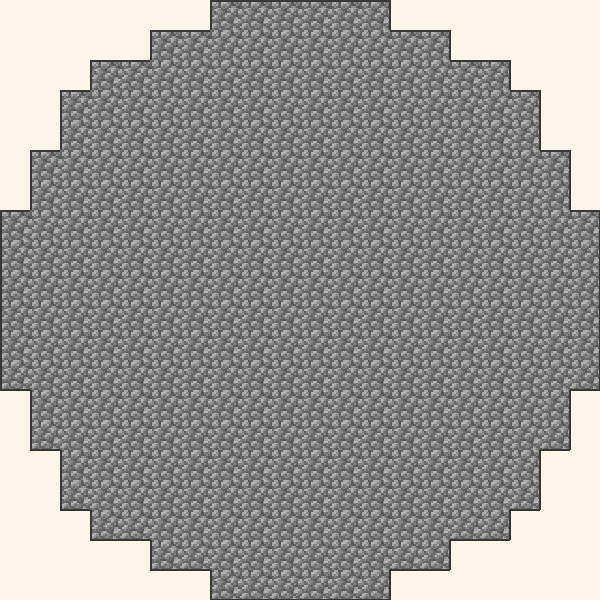
\includegraphics[width=\linewidth]{fig04_2d_d20_euclidean.png}
  \caption{\emph{Евклидов}}
\end{subfigure}\hfill
\begin{subfigure}[t]{0.31\linewidth}\centering
  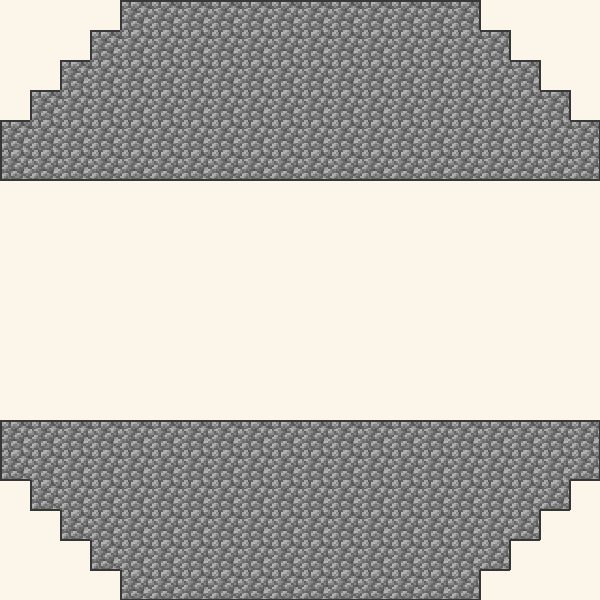
\includegraphics[width=\linewidth]{fig05_2d_d20_bresenham.png}
  \caption{\emph{Брезенхэма}}
\end{subfigure}\hfill
\begin{subfigure}[t]{0.31\linewidth}\centering
  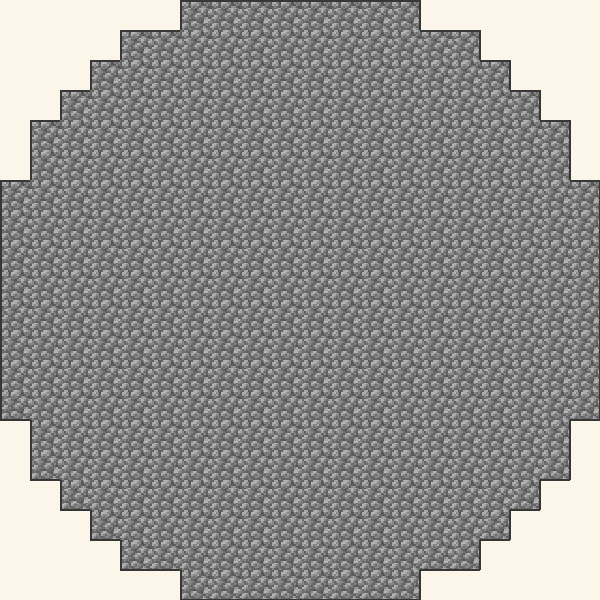
\includegraphics[width=\linewidth]{fig06_2d_d20_threshold.png}
  \caption{\emph{Пороговый}}
\end{subfigure}
\caption{Одна и та же окружность диаметра 20 в трёх алгоритмах с текстурой булыжника. Увеличение диаметра делает различия более тонкими --- три версии выглядят почти одинаково на глаз. Это хороший момент, чтобы напомнить: при меньших диаметрах (рис.~\ref{fig:comp-d10}) различия гораздо заметнее.}
\label{fig:comp-d20}
\end{figure}

\begin{minecraft}[Сравнение количества блоков: Block Round против WorldEdit]
Попробуйте дома (если у вас стоит Minecraft + WorldEdit): выполните \cmd{//sphere stone 10} на сервере и посчитайте блоки. Сравните с тем, что Block Round показывает в \emph{Info chip} для алгоритма Брезенхэма при $D = 20$. Два значения должны совпасть (\emph{или} различаться на 0--4 блока из-за мелких различий в реализации). Если найдёте устойчивое расхождение --- вы обнаружили подлинное математическое любопытство, достойное обсуждения на уроке или даже короткой исследовательской работы.
\end{minecraft}

% =============================================================================
\subsection{Урок 3 --- «От эллипса к эллипсоиду: третье измерение»}\label{aula3}

\subsubsection*{Цель урока}
Обобщить уравнение эллипса на эллипсоид, ввести воксели, вычисление дискретного объёма и плоскостные сечения. Установить связи с визуальным наследием русского авангарда, с традиционной архитектурой коренных народов России и со знаменитыми постройками русскоязычного Minecraft-сообщества.

\begin{zadanie}[3.1 --- От 2D-уравнения к 3D \quad\tempo{15 мин}]\label{at:31}
Добавить третью координату $z$ к декартовой плоскости. Неявное уравнение эллипса естественно обобщается:

\begin{formula}
\centering
$\displaystyle \left(\dfrac{x}{r_x}\right)^{\!2} + \left(\dfrac{y}{r_y}\right)^{\!2} + \left(\dfrac{z}{r_z}\right)^{\!2} \;=\; 1$
\end{formula}

Когда $r_x = r_y = r_z = r$, восстанавливается \acc{сфера} $x^2 + y^2 + z^2 = r^2$, как показано на рис.~\ref{fig:3d-shapes}.

\textbf{Воксели:} клетка трёхмерной сетки называется \emph{вокселем} (\emph{volume element}). В Minecraft каждый воксель соответствует \emph{блоку} $1\times1\times1$. Критерий принадлежности в точности тот же, что в 2D, с добавлением координаты $z$:

\begin{formula}
\centering
$\displaystyle a_x^2 + a_y^2 + a_z^2 \leq 1,\quad \text{где } a_\xi = \dfrac{\xi + \tfrac{1}{2} - c_\xi}{r_\xi}$
\end{formula}

\textbf{Демонстрация:} открыть Block Round в режиме 3D, переключаться между Сферой и Эллипсоидом, вращать мышью, наблюдать воксельную структуру.
\end{zadanie}

\begin{figure}[!htbp]
\centering
\begin{subfigure}[t]{0.45\linewidth}\centering
  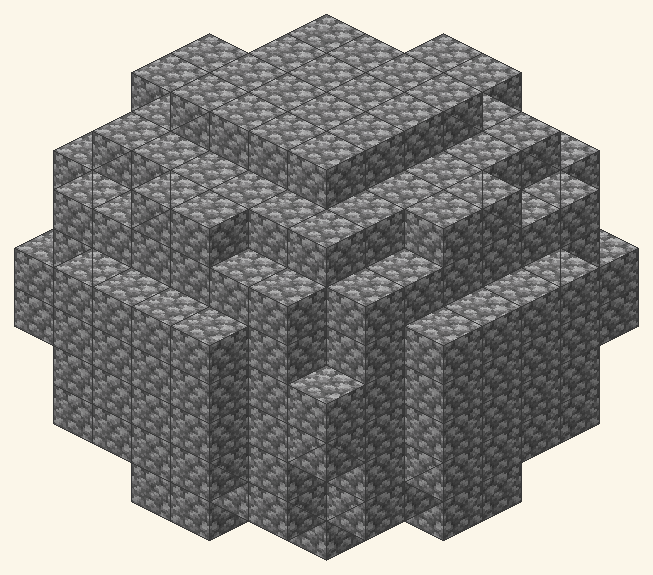
\includegraphics[width=\linewidth]{fig10_3d_sphere_d12.png}
  \caption{Сфера диаметра 10 ($r_x = r_y = r_z = 5$).}
\end{subfigure}\hfill
\begin{subfigure}[t]{0.45\linewidth}\centering
  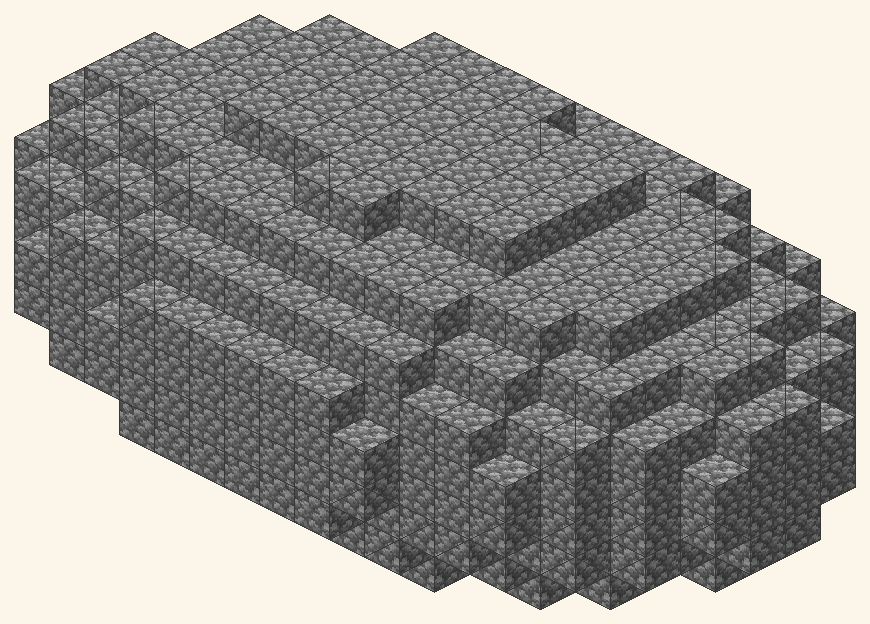
\includegraphics[width=\linewidth]{fig11_3d_ellipsoid.png}
  \caption{Эллипсоид с $W = 20, H = 10, D = 12$.}
\end{subfigure}
\caption{Воксе\-ли\-зация в 3D. Каждый куб --- воксель (т.\,е.\ блок Minecraft); его центральная координата $(i, j, k)$ подставляется в неявное уравнение. Видимые лестничные ступени на поверхности характерны для воксе\-ли\-зации --- именно тот вид, что задаёт Minecraft его узнаваемый визуальный язык.}
\label{fig:3d-shapes}
\end{figure}

\begin{zadanie}[3.2 --- Непрерывный объём против дискретного \quad\tempo{15 мин}]\label{at:32}
Непрерывный объём эллипсоида --- классический результат:

\begin{formula}
\centering
$\displaystyle V \;=\; \dfrac{4}{3}\,\pi\, r_x\, r_y\, r_z$
\end{formula}

Когда $r_x = r_y = r_z = r$, $V = \tfrac{4}{3}\pi r^3$. Это содержание \acc{регулярно встречается на ЕГЭ} (стереометрия в задачах 8 и 14 профильного уровня), а также в задачах второго тура \hyperref[sec:olimp]{ВсОШ}, особенно в задачах на численное приближение и оценку.

\textbf{Задание в паре:}
\begin{enumerate}[leftmargin=1.5em,itemsep=0.15em,topsep=0.3em,nosep]
  \item Вычислить непрерывный объём сферы диаметра 12 ($r = 6$): $V = \tfrac{4}{3}\pi \cdot 216 \approx 904{,}78$.
  \item В Block Round сгенерировать сферу $D = 12$, режим \emph{Заполненный}, нажать \emph{Info chip}, записать дискретный объём (число блоков): приблизительно $V_{\mathrm{disc}} \approx 904$ блоков. \emph{Относительная погрешность $\approx 0{,}1\,\%$ --- впечатляющая точность.}
  \item В этом же чипе обратить внимание на запись \emph{$904 = 14 \times 64 + 8$}: игра сообщит строителю выживания --- «вам нужно \emph{14 полных стаков} булыжника + один частичный стак с \emph{8 блоками}».
  \item Повторить для $D = 16$ ($V_{\mathrm{cont}} \approx 2\,144$; $V_{\mathrm{disc}} \approx 2\,145$). Заметить, что для чётного $D$ погрешность может быть даже \emph{положительной} (переоценка из-за центра между клетками).
\end{enumerate}

\textbf{Замечание:} отношение $\text{дискр.\ объём}/\text{непрер.\ объём} \to 1$ при $D \to \infty$. Для малых $D$ есть заметное расхождение --- и это математически корректно: дискретизация \emph{действительно} меняет подсчёт. Это, по сути, идея интеграла Римана: дискретные суммы по сетке сходятся к интегралу, и сходимость можно изучить количественно.
\end{zadanie}

\begin{zadanie}[3.3 --- Сечения плоскостями \quad\tempo{10 мин}]\label{at:33}
Block Round позволяет резать эллипсоид по трём разным плоскостям. Каждое сечение --- это \acc{линейное неравенство}, применённое к центру вокселя:

\begin{formula}
\centering
$\begin{array}{lcl}
\text{Ось X:} & x \geq \mathit{cut} & \Rightarrow \text{воксель отбрасывается} \\
\text{Ось Y:} & y \geq \mathit{cut} & \Rightarrow \text{воксель отбрасывается} \\
\text{Диагональ:} & x + y \geq \mathit{cut} & \Rightarrow \text{воксель отбрасывается}
\end{array}$
\end{formula}

Рис.~\ref{fig:cortes} показывает три сечения при $50\,\%$.

\textbf{Направляемое обсуждение:} \emph{«Почему у диагонального сечения амплитуда $D_x + D_y$, а не $D_x$? Где гипотенуза?»} Подвести к признанию, что $x + y$ принимает значения от $0$ до $D_x + D_y$ на прямоугольной рамке. \emph{В Minecraft срез Y 50\,\% сферы даёт классический «купол» --- верхняя половина сферы, ровно то, что покрывает храмы, обсерватории и арены на тысячах серверов.}
\end{zadanie}

\begin{figure}[!htbp]
\centering
\begin{subfigure}[t]{0.31\linewidth}\centering
  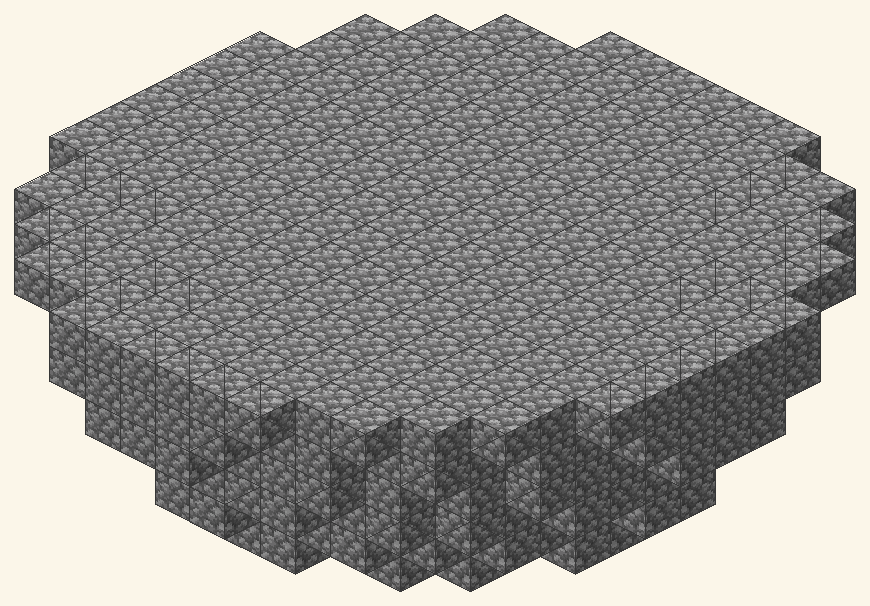
\includegraphics[width=\linewidth]{fig12_3d_cut_y50.png}
  \caption{Срез Y на 50\,\% --- классический \emph{купол}.}
\end{subfigure}\hfill
\begin{subfigure}[t]{0.31\linewidth}\centering
  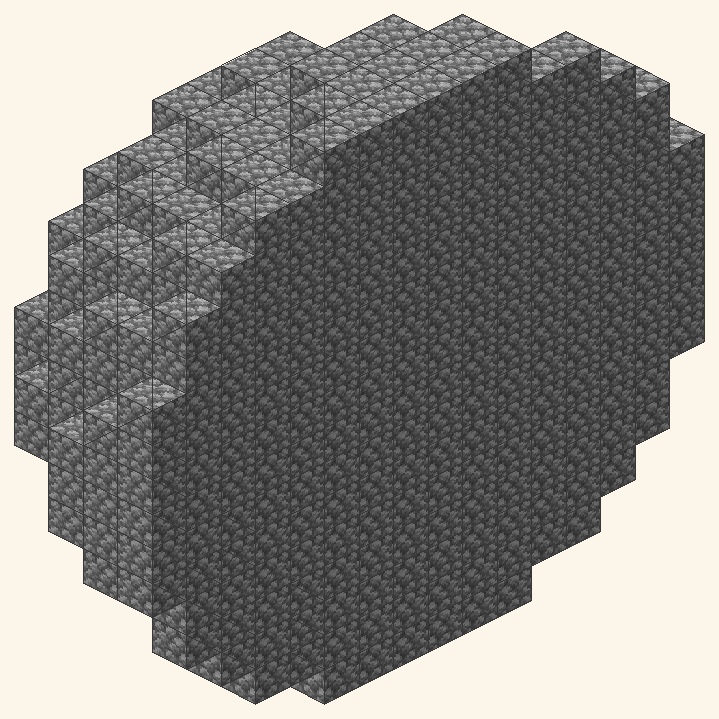
\includegraphics[width=\linewidth]{fig13_3d_cut_x50.png}
  \caption{Срез X на 50\,\% --- \emph{боковая полусфера}.}
\end{subfigure}\hfill
\begin{subfigure}[t]{0.31\linewidth}\centering
  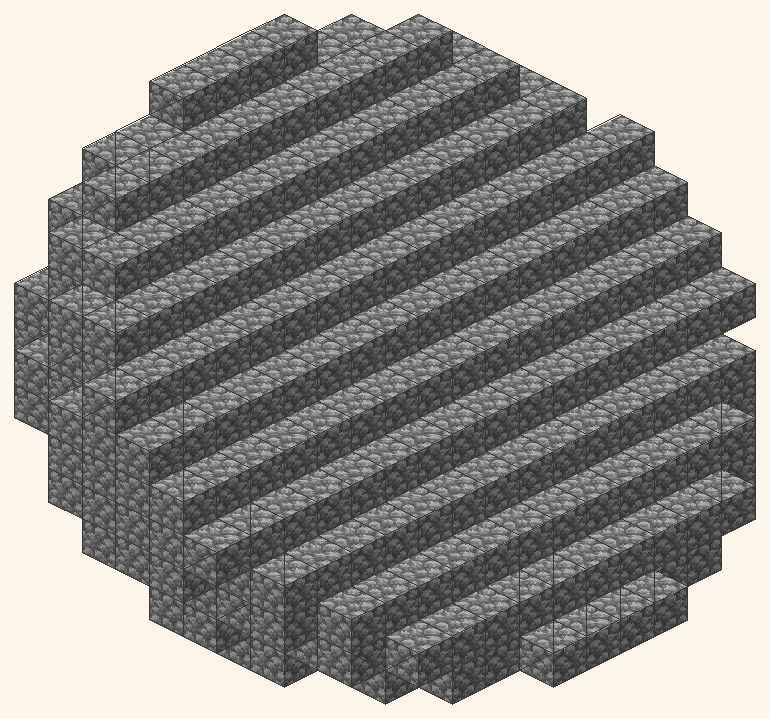
\includegraphics[width=\linewidth]{fig14_3d_cut_diag50.png}
  \caption{Диагональный срез на 50\,\% --- \emph{косая полу\-чаша}.}
\end{subfigure}
\caption{Три плоскостных сечения одного и того же эллипсоида диаметра 16, каждое сохраняющее $50\,\%$ объёма. Заметьте характерный ступенчатый узор диагонального сечения: он обнажает гипотенузу, соединяющую две оси. Каждое сечение --- это другой план постройки в Minecraft: храмовый купол, боковая полу-арена, амфитеатр с фонтаном.}
\label{fig:cortes}
\end{figure}

\begin{zadanie}[3.4 --- Диалог с визуальным наследием России \quad\tempo{10 мин}]\label{at:34}
\emph{Связь с изобразительным искусством, литературой и историей. Это задание реализует метапредметные результаты ФГОС СОО о культурной идентичности и наследии.}

Спроецировать (или раздать в распечатанном виде) пять изображений:

\begin{itemize}[leftmargin=1.3em,itemsep=0.2em,topsep=0.3em,nosep]
  \item \acc{Шуховская башня на Шаболовке} (В. Г. Шухов, 1922): её металлическая конструкция в форме \emph{гиперболоида вращения} --- прямая инженерная реализация той математической поверхности, что мы изучаем. Шухов высотой 160 метров рассчитал оптимальную геометрию из прямолинейных стальных сегментов, образующих кривую поверхность. Это \emph{та самая математика}, что лежит за уравнением эллипсоида --- семейство квадрик. Также можно показать водонапорные башни Шухова в Полибино и Аджигиоле.

  \item \acc{Чум ненцев, яранга чукчей и юрта алтайцев/якутов}: традиционные жилища коренных народов России обладают круговой и сферической геометрией. Знание о том, как именно надо натянуть оленьи шкуры на конический каркас чума или войлок на полусферический каркас юрты, передавалось из поколения в поколение веками. Это сложная геометрия --- \emph{воксе\-ли\-зация}, хотя без формального имени.

  \item \acc{Русский авангард --- К. С. Малевич «Чёрный квадрат» (1915), Эль Лисицкий «Клин красным» (1919), В. Е. Татлин «Памятник III Интернационалу» (Башня Татлина, 1919--20)}: целое поколение русских художников, на сто лет опередивших Minecraft, работали именно с геометрической формой как первоэлементом искусства. Малевич и его супрематизм --- это, по сути, манифест воксельного и пиксельного искусства за столетие до его технологического воплощения. Башня Татлина в форме спирального гиперболоида никогда не была построена в металле, но в истории мирового искусства занимает место одной из самых известных нереализованных идей.

  \item \acc{Кижи --- ансамбль деревянного зодчества Карелии, объект Всемирного наследия ЮНЕСКО}: 22 купола Преображенской церкви на острове Кижи (1714 год). Также: храм Василия Блаженного в Москве (Покровский собор, 1561) --- его луковичные купола представляют собой сложные поверхности вращения, близкие к эллипсоиду. Софийский собор в Великом Новгороде (1045--50). \emph{Это и есть русская геометрия в дереве и камне за столетия до информатики.}

  \item \acc{Постройки русскоязычного Minecraft-сообщества}: города на серверах GhostCraft, Crystal-MC, MineFun, Polar Network; реконструкции Кремля Москвы, Эрмитажа, Большого театра в Minecraft, активно публикуемые на YouTube такими блогерами как TheBrainDit, EvgenBro, Frost Bee, FILIPIN, Compot, Олег Брейн. Можно показать таймлапсы строительства куполов, сфер и арок. \emph{Это и есть русскоязычная Minecraft-этно\-мате\-ма\-тика в действии}, современная, живая, на русском языке.
\end{itemize}

\textbf{Направляемое обсуждение:} \emph{«Шухов рассчитал и построил в металле те же поверхности, что вы нарисовали в блоках. Малевич, Лисицкий и Татлин превратили геометрию в искусство в первой четверти XX века --- задолго до компьютеров. Кижские мастера и палехские иконописцы веками владели сложной геометрией орнамента. Коренные народы Севера складывали полусферические юрты из оленьих шкур, передавая знание от деда к внуку. Русскоязычное Minecraft-сообщество делает это сегодня, живьём, на общих серверах. Задача дискретной растеризации, которую мы изучаем, --- не изобретение цифровой эпохи: это константа человеческой истории. Каждая культура нашла свой способ \emph{растеризовать}.»}

\textbf{Межпредметные связи:} предлагается партнёрство с учителем изобразительного искусства, истории и/или географии для углубления темы. Урок~\ref{aula4} и Урок~\ref{aula5} могут потребовать от групп \emph{выбрать}, какая визуальная традиция России вдохновит их работу.
\end{zadanie}

% =============================================================================
\subsection{Урок 4 --- «Арифметика инвентаря: стаки, сундуки, команды»}\label{aula4}

\subsubsection*{Цель урока}
Ввести \emph{арифметику инвентаря} Minecraft как конкретное применение деления с округлением вверх и представления частного и остатка. Представить ключевые команды (\cmd{/fill}, \cmd{/clone}, \cmd{//sphere}, \cmd{//hsphere}) и оптимизацию через октаэдрическую симметрию.

\begin{zadanie}[4.1 --- Арифметика стаков \quad\tempo{15 мин}]\label{at:41}
В Minecraft каждая ячейка инвентаря вмещает не более \acc{64 одинаковых блоков}. Этот предел и придаёт практический смысл вычислению объёма: $V = 904$ блока для сферы $D=12$ \emph{не означает} «904 в сумке» --- означает «$\lceil 904/64 \rceil = 15$ \emph{стаков} (полных ячеек)» булыжника.

\textbf{Ключевые формулы:}

\begin{formula}
\centering
$\displaystyle N_{\mathrm{стаков}} = \left\lceil \dfrac{V}{64} \right\rceil
\qquad\qquad
N_{\mathrm{дв.\,сундуков}} = \left\lceil \dfrac{V}{3\,456} \right\rceil$
\end{formula}

(Обычный сундук имеет 27 ячеек; двойной --- 54; $54 \times 64 = 3\,456$ предметов в двойном сундуке.)

\textbf{Задание в паре:}
\begin{enumerate}[leftmargin=1.5em,itemsep=0.15em,topsep=0.3em,nosep]
  \item Для сферы $D = 8$ (объём $\approx 268$ блоков): сколько стаков? Сколько обычных сундуков? Ответ: 5 стаков; 1 обычный сундук (17 свободных ячеек).
  \item Для сферы $D = 16$ (объём $\approx 2\,145$ блоков): сколько стаков? Сколько двойных сундуков? Ответ: 34 стака; 1 двойной сундук (не хватает 20 стаков до заполнения --- то есть остаётся место ещё на маленький цилиндр).
  \item Для сферы $D = 32$ (объём $\approx 17\,156$ блоков): сколько стаков? Сколько двойных сундуков? Ответ: 269 стаков ($\approx 5$ двойных сундуков $+$ 1 стак), $\lceil 17\,156/3\,456 \rceil = 5$ двойных сундуков.
  \item \emph{В Minecraft, в режиме выживания, шахтёры обычно добывают 1 стак булыжника каждые 4--6 минут (зависит от качества кирки). Подсчитать общее время добычи материала для сферы $D = 16$: $34 \times 5 = 170$ минут $\approx 2{,}8$ часа.}
\end{enumerate}
\end{zadanie}

\begin{zadanie}[4.2 --- Команды Minecraft \quad\tempo{15 мин}]\label{at:42}
Представить центральные команды:

\begin{itemize}[leftmargin=1.4em,itemsep=0.25em,topsep=0.3em]
  \item \cmd{/setblock x y z minecraft:stone} --- ставит блок в конкретную позицию.
  \item \cmd{/fill x1 y1 z1 x2 y2 z2 minecraft:stone} --- заполняет прямоугольную область выбранным блоком. Ванильный лимит: $32\,768$ блоков на одну команду.
  \item \cmd{/clone x1 y1 z1 x2 y2 z2 x3 y3 z3} --- копирует область в другую позицию (фундаментальная сила для построек по симметрии).
  \item \cmd{//sphere stone 8} (WorldEdit) --- рисует сферу радиуса 8 с центром в позиции игрока, используя 3D-Брезенхэма.
  \item \cmd{//hsphere stone 8} (WorldEdit) --- рисует \emph{пустую} сферу (только оболочку). Полезно для куполов с пустотой внутри.
  \item \cmd{//ellipsoid stone 10 5 10} (WorldEdit) --- эллипсоид $W = 20, H = 10, D = 20$ с указанными полуосями.
\end{itemize}

\textbf{Демонстрация (при наличии Minecraft):} выполнить \cmd{//sphere stone 8} в тестовом мире и засечь время. Сравнить с тем, что Block Round показывает для диаметра 16, алгоритма Брезенхэма. Подтвердить математическую идентичность двух результатов.

\textbf{Если Minecraft недоступен:} выполнить мысленно. Записать на клетчатой бумаге: «Я стою на земле (y=64). Хочу сферу радиуса 8, начиная с y=72 (на 8 блоков выше земли). Какая команда?» Ответ: \cmd{//sphere stone 8}, стоя в $(0, 72, 0)$.
\end{zadanie}

\begin{zadanie}[4.3 --- Оптимизация через октаэдрическую симметрию \quad\tempo{15 мин}]\label{at:43}
\textbf{Центральная идея:} сфера, центрированная в начале координат, инвариантна относительно отражений в трёх координатных плоскостях. Группа $\mathbb{Z}_2^3$ имеет порядок 8: из одного \emph{октанта} (область $+x, +y, +z$) семь остальных получаются отражениями.

\textbf{Практическое следствие:} вместо размещения $V$ блоков по одному, построить $V/8$ блоков в положительном октанте и отразить 7 раз командой \cmd{/clone}.

\begin{formula}
\centering
$\displaystyle \mathrm{цена}_\mathrm{симметрия} = N_\mathrm{октант} + 7\, T_\mathrm{clone}
\;\ll\; \mathrm{цена}_\mathrm{полный\,перебор} = N\, T_\mathrm{блок}$
\end{formula}

\textbf{Конкретный пример, сфера $D = 24$ с центром в $(0, 72, 0)$:}
\begin{enumerate}[leftmargin=1.5em,itemsep=0.15em,topsep=0.3em,nosep]
  \item Построить вручную положительный октант ($\approx 905$ блоков, $\approx 15$ минут в выживании или $\approx 45$ секунд в творческом режиме с кистью).
  \item Отразить в $-x$: \cmd{/clone 0 72 0 12 84 12 -12 72 0 mode:masked}
  \item Отразить в $-y$: \cmd{/clone 0 72 0 12 84 12 0 60 0 mode:masked}
  \item Отразить в $-z$: \cmd{/clone 0 72 0 12 84 12 0 72 -12 mode:masked}
  \item Октанты $(-x, -y)$, $(-y, -z)$, $(-x, -z)$, $(-x, -y, -z)$: аналогичные команды.
\end{enumerate}

\textbf{Сравнение времени:}
\begin{itemize}[leftmargin=1.3em,itemsep=0.1em,topsep=0.2em,nosep]
  \item Без симметрии, в выживании: $7\,238$ блоков $\times$ 2\,с/блок $\approx$ 4 часа.
  \item С симметрией: 15 мин (октант) + 0{,}5\,с (7 клонов) $\approx$ 15 мин.
  \item Ускорение: \emph{в 16 раз}.
\end{itemize}
\end{zadanie}

\begin{zadanie}[4.4 --- Прикладная задача: планирование настоящего купола \quad\tempo{5 мин}]
В парах спланировать (\emph{на бумаге или в Block Round}) строительство купола из Quartz $D=20$ над храмом, оформленным в стиле русского православного собора, шуховской башни или коренной северной архитектуры. Записать:
\begin{itemize}[leftmargin=1.3em,itemsep=0.1em,topsep=0.2em,nosep]
  \item Объём купола (половина сферы $D=20$): $\approx 2\,094$ блока.
  \item Необходимые стаки: 33 стака.
  \item Число блоков Quartz (каждый требует 4 Nether Quartz, добываемого в Нижнем мире): $\sim 2\,094 \times 4 = 8\,376$ Nether Quartz.
  \item Оптимизированная последовательность команд с использованием симметрии.
\end{itemize}

Это задание подготавливает почву для Урока 5 (реальное строительство).
\end{zadanie}

% =============================================================================
\subsection{Урок 5 --- «Реальное строительство: от Block Round к Minecraft»}\label{aula5}

\subsubsection*{Цель урока}
Мобилизовать всё развернутое содержание в \emph{авторском построенном произведении}: экспорт из Block Round, импорт в Minecraft (через Litematica или Schematica), выполнение постройки в творческом или выживальном режиме. Оценить обучение через защитную аргументацию математических решений и сдачу финального продукта.

\begin{zadanie}[5.1 --- Представление вызова \quad\tempo{5 мин}]\label{at:51}
\textbf{Команда:} \emph{«В парах или тройках вы создадите постройку в Minecraft (или в Block Round, если Minecraft недоступен), сочетающую как минимум три фигуры, сгенерированные Block Round (окружности, эллипсы, сферы или эллипсоиды). Это может быть город на сервере класса, храм, круглая ферма, обсерватория --- выбираете вы. В конце каждая группа представит работу, объясняя \acc{математически} выбор: почему именно этот алгоритм? почему такая пропорция? почему такой срез? почему такие блоки?»}
\end{zadanie}

\begin{zadanie}[5.2 --- Экспорт и импорт \quad\tempo{15 мин}]\label{at:52}
Продемонстрировать поток Block Round $\rightarrow$ Minecraft:

\begin{enumerate}[leftmargin=1.5em,itemsep=0.2em,topsep=0.3em]
  \item В Block Round задать желаемую фигуру (например, сферу $D = 12$ из Quartz со срезом Y 50\,\%).
  \item Нажать кнопку \emph{Export Schematic} в углу холста. Файл \texttt{.schem} (Sponge Schematic v2) скачается.
  \item В Minecraft Java Edition с установленным модом \emph{Litematica} (бесплатный): открыть мод, \emph{Load Schematic}, выбрать скачанный файл.
  \item Litematica показывает полупрозрачный «призрак» постройки в выбранной игроком позиции.
  \item Игрок ставит каждый блок \emph{следуя призраку}. Litematica подсвечивает красным любой блок, поставленный не туда.
  \item \emph{Альтернатива через \cmd{//schem load}:} на сервере с WorldEdit команда \cmd{//schem load имя\_файла} импортирует схему, а \cmd{//paste -a} вставляет её на текущую позицию --- мгновенная постройка.
\end{enumerate}

\textbf{Если Minecraft недоступен:} продемонстрировать экспорт \texttt{.schem} и показать бинарный файл в шестнадцатеричном редакторе --- обсуждение формата Sponge v2, gzip-сжатия, NBT-сериализации. Прямое содержание профильного ЕГЭ по информатике (задача 16 на представление информации).
\end{zadanie}

\begin{zadanie}[5.3 --- Производство \quad\tempo{20 мин}]\label{at:53}
\textbf{Материалы на группу:}
\begin{itemize}[leftmargin=1.3em,itemsep=0.15em,topsep=0.3em,nosep]
  \item Доступ к Block Round (компьютер или \emph{смартфон});
  \item (Опционально) доступ к Minecraft с Litematica или Schematica;
  \item Клетчатая бумага, карандаш и фломастеры для эскизов и сценария;
  \item Лист-сценарий с тремя обязательными вопросами (Приложение~\ref{ap:exerc}, упражнение 8).
\end{itemize}

\textbf{Внутренние этапы групповой работы:}
\begin{enumerate}[leftmargin=1.5em,itemsep=0.15em,topsep=0.3em,nosep]
  \item \tempo{5 мин} Мозговой штурм и эскиз на бумаге.
  \item \tempo{8 мин} Создание в Block Round и экспорт \texttt{.schem}.
  \item \tempo{5 мин} Импорт в Minecraft и быстрый тест (если доступно).
  \item \tempo{2 мин} Запись математического обоснования в сценарии.
\end{enumerate}

\textbf{Учительское сопровождение:} обходить группы, задавать вопросы-провокации --- \emph{«Почему вы выбрали именно этот алгоритм? Как этот срез можно описать неравенством? Сколько двойных сундуков Quartz вам понадобится?»}
\end{zadanie}

\begin{zadanie}[5.4 --- Защита и коллективный синтез \quad\tempo{10 мин}]\label{at:54}
Каждая группа располагает 2 минутами для представления работы классу: показывая её на проекторе (или в Minecraft, или физически на бумаге) и отвечая \emph{по меньшей мере на один} из трёх обязательных математических вопросов.

\textbf{Минимальные критерии защиты:}
\begin{itemize}[leftmargin=1.3em,itemsep=0.1em,topsep=0.2em,nosep]
  \item опознать хотя бы одну геометрическую фигуру в работе;
  \item назвать выбранный алгоритм и обосновать (хотя бы \emph{постфактум}) его соответствие желаемому визуальному эффекту;
  \item если есть 3D-срез, описать его как неравенство;
  \item оценить (хотя бы приблизительно) число стаков/сундуков, необходимых в выживании.
\end{itemize}

\textbf{Итоговый синтез учителем (3 мин):} вернуться к центральной идее последовательности --- \emph{«на дискретной сетке вокселей одна и та же непрерывная кривая допускает множество представлений; выбор одного из них --- это математическое решение; построение этого в Minecraft --- это решение о гражданственности, управлении ресурсами и эстетике»} --- и поместить её в горизонт современной русской математики: пригласить класс изучить \hyperref[sec:olimp]{ВсОШ}, узнать о Г. Я. Перельмане и о русских математиках, получивших Филдсовскую медаль (С. П. Новиков, Г. А. Маргулис, В. Г. Дринфельд, Е. И. Зельманов, М. Л. Концевич, В. А. Воеводский, А. Ю. Окуньков, Г. Я. Перельман, С. К. Смирнов), а также присоединиться к российским серверам Minecraft, продвигающим коллективные строительные проекты.
\end{zadanie}

\begin{minecraft}[Возможности расширения]
Этот Урок 5 открывает несколько возможностей для внеурочного расширения:
\begin{itemize}[leftmargin=1.3em,itemsep=0.15em,topsep=0.3em,nosep]
  \item \textbf{Проект «Математический город»:} класс строит на школьном сервере город, в котором каждое здание реализует геометрическую фигуру (цилиндр, сфера, эллипсоид, набор кривых второго порядка).
  \item \textbf{Реконструкция культурного наследия России:} воспроизведение в Minecraft Шуховской башни, храма Василия Блаженного, ансамбля Кижи, Большого театра, башни «Лахта-Центра» (Санкт-Петербург, 462 м), Останкинской телебашни, главного здания МГУ на Воробьёвых горах (сталинская архитектура), Соловецкого монастыря, чума ненцев или яранги чукчей.
  \item \textbf{Олимпиада Block Round:} внутренний конкурс --- кто построит сферу, ближайшую к непрерывному объёму? кто оптимизирует время через симметрию?
  \item \textbf{Связь с инженерией (СУНЦ и физматлицеи):} использовать Block Round как песочницу пред-инженерии: геодезические купола, воксе\-ли\-зированные фермы, конструкции, аппроксимирующие гладкие поверхности.
  \item \textbf{Связь с информатикой (ВсОШ по информатике):} переписать три алгоритма на Python или Scratch, сравнить выходы с Block Round, представить анализ как индивидуальный учебный проект 11 класса (один из обязательных элементов программы выпускного класса).
\end{itemize}
\end{minecraft}

% =============================================================================
\section{Оценивание}\label{sec:avaliacao}

Оценивание следует \acc{формирующей}, \acc{процессуальной} и \acc{итоговой} моделям, объединяя четыре измерения (плюс особое измерение для Minecraft-применения) и опираясь на отечественную традицию критериального оценивания (М. А. Пинская, А. Б. Воронцов и др.), а также на работы НИУ ВШЭ по образовательному измерению.

\subsection{Диагностическое оценивание}
Проводится в Уроке~\ref{aula1}, в момент Задания~1.2 (ручное построение круга). Позволяет учителю выявить трудности с декартовой системой координат, уравнением окружности и счётом --- и компенсировать постпандемические пробелы, отмеченные в исследованиях ВПР и НИКО.

\subsection{Формирующее оценивание}
Распределено по пяти урокам: прямое наблюдение участия, качество ответов в \emph{think--pair--share}, \emph{немедленная} коррекция вычислений в заданиях~\ref{at:25}, \ref{at:32} и~\ref{at:41}.

\subsection{Итоговое оценивание}
Состоит из двух сдач:

\begin{enumerate}[leftmargin=1.5em,itemsep=0.2em,topsep=0.3em,nosep]
  \item \textbf{Список упражнений} (Приложение~\ref{ap:exerc}), 8 задач, сдаётся в конце Урока~\ref{aula5} или в согласованную дату.
  \item \textbf{Финальный проект} (Задание~\ref{at:53}), с сценарием, заполненным во время защиты (Задание~\ref{at:54}).
\end{enumerate}

\subsection{Критериальная шкала}

\begin{center}
\small
\begin{tabularx}{\textwidth}{@{}p{0.21\textwidth}XX@{}}
\toprule
\textbf{Критерий} & \textbf{Полностью удовлетворительно (8--10)} & \textbf{Частично удовлетворительно (5--7) / Неудовлетворительно (0--4)} \\
\midrule
\textbf{Математические понятия} & Корректно применяет неявное уравнение эллипса/эллипсоида; распознаёт три алгоритма и их различия. & Применяет базовое уравнение окружности, но путается при обобщении до эллипса / не различает алгоритмы. \\
\addlinespace[3pt]
\textbf{Работа с ПО (Block Round)} & Автономно работает с Block Round в 2D и 3D; экспортирует изображения и \texttt{.schem}; переключает алгоритмы и стили. & Часто нуждается в помощи; работает только в 2D. \\
\addlinespace[3pt]
\textbf{Аргументация} & Математически обосновывает выбор в финальном проекте; использует уместную терминологию (\emph{алгоритм}, \emph{воксель}, \emph{срез}, \emph{неравенство}, \emph{стак}, \emph{двойной сундук}). & Обосновывает только эстетически, не мобилизуя математику; терминология отсутствует. \\
\addlinespace[3pt]
\textbf{Прикладная Minecraft-математика} & Корректно вычисляет стаки и сундуки для проекта; описывает последовательность команд \cmd{/fill} или \cmd{//sphere}; использует октаэдрическую симметрию. & Путает частное и остаток; обрабатывает блоки как отдельные единицы; не пользуется симметрией. \\
\addlinespace[3pt]
\textbf{Сотрудничество} & Продуктивно работает в паре/тройке; вносит вклад в общее обсуждение. & Работает изолированно; вклад минимальный. \\
\bottomrule
\end{tabularx}
\end{center}

\subsection{Перевод в школьные отметки (5-балльная система)}
\begin{itemize}[leftmargin=1.3em,itemsep=0.1em,topsep=0.2em,nosep]
  \item Список упражнений: 40\,\% итоговой оценки.
  \item Финальный проект + защита: 50\,\% итоговой оценки.
  \item Процессуальное наблюдение (участие): 10\,\% итоговой оценки.
  \item Конвертация в традиционную пятибалльную шкалу: 8--10 баллов $\rightarrow$ «отлично» (5); 6--7 $\rightarrow$ «хорошо» (4); 4--5 $\rightarrow$ «удовлетворительно» (3); 0--3 $\rightarrow$ «неудовлетворительно» (2).
\end{itemize}

% =============================================================================
\section{Связи с российской математической экосистемой}\label{sec:olimp}

Эта последовательность вписывается в \emph{богатую экосистему} российских инициатив образования и исследования в области математики и информатики, которые учитель может мобилизовать для расширения и углубления.

\subsection{Всероссийская олимпиада школьников (ВсОШ) по математике}

\href{https://olimpiada.ru/}{Всероссийская олимпиада школьников} (ВсОШ) по математике --- крупнейшая олимпиада России, организуемая Министерством просвещения с 1961 года (как наследница Олимпиад советских школьников). Включает четыре этапа: школьный, муниципальный, региональный и заключительный. Заключительный этап ежегодно собирает несколько сотен сильнейших школьников страны. \emph{Содержание этой последовательности (аналитическая геометрия окружности и эллипсоида, алгоритмическое мышление, численные приближения) непосредственно готовит к задачам регионального и заключительного этапов ВсОШ среди старшеклассников.}

\subsection{Турнир городов и другие олимпиады}

Турнир городов (Tournament of Towns) --- международный матема\-ти\-чес\-кий турнир, основанный в 1980 году в Москве. Имеет особую традицию задач на оценки и приближения. Московская математическая олимпиада. Олимпиада им. Леонарда Эйлера (для 8 класса, как путь подготовки к ВсОШ среди старшеклассников). Также Международная математическая олимпиада (IMO): команда России (унаследовав традицию команды СССР, начавшей участвовать с 1959 года) традиционно входит в число сильнейших.

\subsection{Образовательный центр «Сириус» в Сочи}

\href{https://sochisirius.ru/}{Образовательный центр «Сириус»} (Фонд «Талант и успех») основан в 2014 году по инициативе Президента России для одарённых детей. Проводит летние и осенние смены по математике, физике, информатике, естественным наукам, искусству. Победители ВсОШ и медалисты олимпиад имеют приоритетный доступ. Это естественная точка следующего шага для учащихся, проявивших интерес после этой последовательности уроков. Также: летние школы СУНЦ МГУ имени Колмогорова, СУНЦ НГУ при НГУ, СУНЦ СПбГУ, СУНЦ УрФУ; летние математические школы в Дубне; Заочная математическая школа МГУ, основанная И. М. Гельфандом в 1964 году.

\subsection{Г. Я. Перельман и российская математика}

В 2003 году \acc{Григорий Яковлевич Перельман}, выпускник Ленинградского государственного университета (СПбГУ) и сотрудник Санкт-Петербургского отделения Математического института имени В. А. Стеклова РАН (ПОМИ), опубликовал доказательство \emph{гипотезы Пуанкаре} --- одной из семи Задач тысячелетия. В 2006 году ему была присуждена Филдсовская медаль, от которой он отказался; в 2010 году --- премия Института Клэя в миллион долларов, от которой он также отказался. Перельман --- ярчайший символ силы петербургской математической школы, наследника П. Л. Чебышёва (1821--1894, теория приближений) и А. А. Маркова-старшего (1856--1922, марковские цепи). СССР и Россия дали 10 обладателей Филдсовской медали: С. П. Новиков (1970), Г. А. Маргулис (1978), В. Г. Дринфельд (1990), Е. И. Зельманов (1994), М. Л. Концевич (1998), В. А. Воеводский (2002), А. Ю. Окуньков (2006), Г. Я. Перельман (2006), С. К. Смирнов (2010), и обладатель Абелевской премии 2009 М. Л. Громов. По числу филдсовских медалистов после США (всего три страны имеют больше десяти медалистов) --- это второй результат в мире.

\subsection{Всероссийская олимпиада школьников по информатике и Codeforces}

ВсОШ по информатике организуется Министерством просвещения; победители заключительного этапа получают льготы при поступлении в ведущие технические вузы (МФТИ, МГУ ВМК, ИТМО, СПбГУ, НИУ ВШЭ, МГТУ имени Баумана, НГУ, УрФУ). На региональном уровне традиционно встречаются задачи на дискретную геометрию и графику, тесно связанные с алгоритмом Брезенхэма (рассмотренным в Задании~\ref{at:23}).

Платформа \href{https://codeforces.com}{Codeforces}, созданная в 2009 году командой М. Мирзаянова в Саратовском государственном университете, стала ведущей мировой платформой для соревновательного программирования. На Codeforces проходят раунды от Educational Round до Round Codeforces, доступные на русском и английском языках. ВКОШП (Всероссийская командная олимпиада школьников по программированию) --- ещё одна важная российская традиция.

\subsection{Российская математическая традиция в школе}

В образовании математики в России отдельно стоят имена и школы:

\begin{itemize}[leftmargin=1.3em,itemsep=0.15em,topsep=0.3em]
  \item \acc{Н. И. Лобачевский} (1792--1856), Казань --- неевклидова геометрия. Его работа 1829 года «О началах геометрии» --- первая систематическая публикация неевклидовой геометрии в мире. Любой урок геометрии в российской школе несёт его наследие.
  \item \acc{С. В. Ковалевская} (1850--1891) --- первая женщина-член-корреспондент Российской академии наук, первая женщина-профессор математики в Северной Европе (Стокгольмский университет), лауреат премии Бордена французской Академии наук (1888). Пионер женщин в науке мирового масштаба.
  \item \acc{А. Н. Колмогоров} (1903--1987) --- аксиоматика теории вероятностей (1933, монография «Основные понятия теории вероятностей»). Основал в 1963 году «Колмогоровский интернат», ныне СУНЦ МГУ им. А. Н. Колмогорова. Колмогоров одновременно был великим математиком и крупным реформатором школьного образования 1960--70-х.
  \item \acc{В. И. Арнольд} (1937--2010) --- ученик Колмогорова, лауреат премии Wolf (2001) и многих других. Его учебники по геометрии и дифференциальным уравнениям являются классикой. Известная цитата: «Математика --- это часть физики, в которой эксперимент дёшев».
  \item \acc{И. Ф. Шарыгин} (1937--2004) --- крупнейший методист школьной геометрии в России XX века; автор популярных учебников и задачников.
  \item \acc{И. М. Гельфанд} (1913--2009) --- основатель Заочной математической школы МГУ (1964). Учитель целого поколения математиков мирового уровня.
  \item \acc{Н. Н. Боголюбов} (1909--1992) --- математическая физика, нелинейная механика.
\end{itemize}

\subsection{Математический институт им. В. А. Стеклова РАН и научные центры}

\href{https://www.mathnet.ru/}{Математический институт имени В. А. Стеклова Российской академии наук} (МИАН, Москва, основан в 1934 году) --- ведущий научно-исследовательский центр чистой математики России. Санкт-Петербургское отделение МИАН (ПОМИ) --- где работал Перельман. Независимый московский университет (НМУ) --- математическая школа в Москве, основанная в 1991 году группой ведущих математиков. Математический центр в Академгородке Новосибирска при НГУ. Международный лабораторий по теории струн и математической физике в НИУ ВШЭ. Эти центры представляют живую математическую традицию России, к которой может обратиться выпускник 11 класса при выборе пути дальнейшего обучения.

\subsection{Этноматематика и работы У. Д'Амбросио в русском контексте}

Линия исследования в этноматематике, основанная бразильцем \acc{Убиратаном Д'Амбросио} (1932--2021), получившим премию Феликса Клейна ICMI (2005), известна и в России. На русском языке доступны переводы и обзорные статьи в журналах «Математика в школе», «Вопросы психологии», «Информатика и образование». Российские этноматематики В. Дробышев, А. Степанов и другие изучают математические практики коренных народов Севера, Сибири и Поволжья.

\subsection{Подготовка учителей: магистратура «Учитель математики»}

\href{https://мпгу.рф/}{Московский педагогический государственный университет} (МПГУ) предлагает магистратуру «Учитель математики». Аналогичные программы работают в МГПУ, СПбГУ, ОмГПУ, ТГУ (Томск), КФУ (Казань), УрФУ. Конкурс «Учитель года» (с 1990) и «Учитель года России» имеют отдельную номинацию по математике и информатике. Российский Союз учителей математики --- профессиональное сообщество. Эта дидактическая последовательность может стать основой выпускной квалификационной работы магистра.

% =============================================================================
\section{Межпредметные связи}\label{sec:interdisc}

\subsection{С изобразительным искусством}
Производство \emph{воксельного искусства} традиционно изучается как художественный язык. Block Round открывает редкую возможность объединить математику и искусство в одном объекте: фигура \emph{одновременно} является уравнением и эстетической композицией. Предлагается партнёрство с учителем изобразительного искусства для итоговой выставки работ на стенде или в школьных социальных сетях (ВКонтакте, Сферум). Возможное углубление: исследование произведений \emph{русского авангарда} --- К. С. Малевич («Чёрный квадрат», 1915, манифест супрематизма), Эль Лисицкий («Клин красным», 1919), В. В. Кандинский (геометрические абстракции и Баухаус), В. Е. Татлин (Башня Татлина, спиральный гиперболоид), Любовь Попова, Александр Родченко (конструктивизм). Также: формализм ОПОЯЗ (В. Шкловский, Ю. Тынянов, Б. Эйхенбаум) --- их теория «остранения» как геометрия восприятия. Народные геометрические узоры: палехская миниатюра, гжель, хохлома, вологодское кружево, скань (филигрань), вышивка крестом (\emph{прямой воксельный код!}), рукоделие народов Кавказа.

\subsection{С физикой и информатикой}
Звуковой слой Block Round использует аддитивный синтез синусоидальных волн (аналогично Pixel Round). Выбираемые частоты приближаются к нотам \acc{равномерно-темперированного 12-тонального строя} (каждый полутон умножает частоту на $2^{1/12} \approx 1{,}0595$). Содержание связано с \emph{механическими волнами}, \emph{акустикой} и \emph{показательными функциями}. В Minecraft --- связь с \emph{редстоуном} (цифровая логика, прямой аналог булевой алгебры), \emph{нотными блоками}, \emph{физикой жидкостей и сыпучих тел} (песок, гравий, вода). А. Я. Хинчин (теория информации) и А. Н. Колмогоров (формализация теории вероятностей) создали основу того, что сегодня называют теорией информации Шеннона, --- именно эта математика обеспечивает работу цифровых сигналов в любом современном компьютере.

\subsection{С информатикой (профильный курс)}
Алгоритм Брезенхэма --- классическая ссылка в курсе информатики. Связан с уроками \emph{вычислительного мышления}: \emph{абстракция} (уравнение как модель), \emph{декомпозиция} (форма как множество вокселей), \emph{распознавание паттернов} (симметрии), \emph{алгоритмизация} (три процедуры). Прямая связь с \hyperref[sec:olimp]{ВсОШ по информатике} и с углублёнными курсами «Информатика и программирование», доступными в специализированных школах и СУНЦ. С 2019 года Министерство просвещения совместно с НТИ (Национальная технологическая инициатива) реализует программу технопарков «Кванториум», где школьники могут заниматься программированием, 3D-моделированием и робототехникой бесплатно. Генерация \texttt{.schem} (формат Sponge v2 с gzip + NBT) --- \emph{учебный пример} бинарной сериализации --- содержание профильных курсов по системам обработки информации.

\subsection{С историей}
Брезенхэм опубликовал свой алгоритм в 1965 году, в разгар эры компьютеров \emph{мейнфрейм} IBM. В тот же период советская компьютерная наука переживала расцвет: \emph{МЭСМ} С. А. Лебедева (1951, Киев) --- первая советская ЭВМ; \emph{Сетунь} Н. П. Брусенцова (1958, МГУ) --- единственный массовый троичный компьютер в мире; \emph{БЭСМ-6} (1968, Москва) --- самая мощная ЭВМ Европы своего времени; \emph{Эльбрус} Б. А. Бабаяна (1970-е, ИТМ и ВТ). В 1962 году В. М. Глушков из Института кибернетики в Киеве предложил \emph{ОГАС} --- общегосударственную автоматизированную систему, фактически предтечу интернета (за 7 лет до ARPANET!). А. П. Ершов из Новосибирска создал советскую школу теоретического программирования. В 1984 году в Москве Алексей Пажитнов изобрёл \emph{Тетрис} --- одну из первых массовых игр в истории, \emph{и фактически воксельное искусство ещё до Minecraft}. \emph{Minecraft появился в 2009 году, был продан Microsoft в 2014 за 2{,}5 млрд долларов и к 2023 году достиг 300+ миллионов проданных копий, став самой продаваемой видеоигрой в истории.} Современные российские суперкомпьютеры: «Ломоносов-2» при МГУ. Корпоративный сектор: «Лаборатория Касперского» (основана в 1997), «Яндекс» (тоже 1997) --- мировые лидеры в своих нишах. Траектория всех этих технологий пересекается с историей школьного образования и с появлением школьной информатики в России в 1985 году по инициативе А. П. Ершова.

\subsection{С географией}
Растеризация --- не только тема \emph{воксельного искусства}: это основа \emph{геоинформационных систем} (ГИС, GIS). Цифровые карты, спутниковые снимки (российская программа \emph{Канопус-В} наблюдения Земли; российские спутники Роскосмоса), мониторинг лесов и ледников, Государственная геоинформационная система (ФГИС), Российский глобальный навигационный сервис \emph{ГЛОНАСС} (российский аналог GPS, в эксплуатации с 1995, окончательно развёрнут в 2010) --- современные российские примеры той же математической задачи, что разбирается в последовательности. ГЛОНАСС --- это, по сути, глобальная воксельная навигация: разбиение пространства Земли на дискретные ячейки с известными координатами.

\subsection{С инженерией}
Minecraft \emph{активно} используется в российских технических вузах и в их школах при себе (МГТУ им. Н. Э. Баумана; ИТМО Санкт-Петербург, в 2009--2012 годах студенты ИТМО выигрывали ICPC --- чемпионат мира по программированию; МФТИ Долгопрудный; СПбГПУ Петра Великого; НГТУ Новосибирск; УрФУ Екатеринбург) как песочница пред-инженерии: студенты моделируют города, электрические системы через редстоун, гидравлические системы с водой, механические системы с поршнями и наблюдателями. Воксельная геометрия, представленная в этой последовательности, --- это \emph{ментальная математика} для любого, кто будет изучать сопромат, теоретическую механику или строительные конструкции. Олимпиада НТИ (Национальная технологическая инициатива) и WorldSkills Russia (в направлениях программирования, прототипирования, аэрокосмической инженерии) являются естественным продолжением для интересующихся учеников.

% =============================================================================
\section{Список литературы}\label{sec:referencias}

\subsection{Педагогика и образование в России}
\begin{itemize}[leftmargin=1.3em,itemsep=0.15em,topsep=0.3em]
  \item Ушинский К. Д. \emph{Человек как предмет воспитания. Опыт педагогической антропологии}. М.: Педагогика, 1868 (репринт 1948).
  \item Выготский Л. С. \emph{Мышление и речь}. М.: Лабиринт, 1934 (изд. 1999).
  \item Леонтьев А. Н. \emph{Деятельность. Сознание. Личность}. М.: Политиздат, 1975.
  \item Давыдов В. В. \emph{Виды обобщения в обучении: логико-психологические проблемы построения учебных предметов}. М.: Педагогическое общество России, 1972 (переизд. 2000).
  \item Эльконин Д. Б. \emph{Психология игры}. М.: Педагогика, 1978.
  \item Макаренко А. С. \emph{Педагогическая поэма}. М.: ИТРК, 1933--35 (изд. 2003).
  \item Сухомлинский В. А. \emph{Сердце отдаю детям}. Киев: Радянська школа, 1969.
  \item Шарыгин И. Ф. \emph{Геометрия. 7--11 классы}. М.: Дрофа, 2000.
  \item Колмогоров А. Н. \emph{Математика --- наука и профессия}. М.: Наука, 1988.
  \item Гельфанд И. М., Львовский С. М., Тоом А. Л. \emph{Тригонометрия}. М.: МЦНМО, 2002.
\end{itemize}

\subsection{Международные педагогика и психология (русские переводы)}
\begin{itemize}[leftmargin=1.3em,itemsep=0.15em,topsep=0.3em]
  \item Пиаже Ж. \emph{Психология интеллекта}. СПб.: Питер, 2003 [пер. с французского, ориг.~1947].
  \item Брунер Дж. \emph{Психология познания: за пределами непосредственной информации}. М.: Прогресс, 1977 [пер. с английского].
  \item Дьюи Дж. \emph{Демократия и образование}. М.: Педагогика-Пресс, 2000 [ориг.~1916; первый русский перевод в 1920-е через работы С. Т. Шацкого].
  \item Фрейре П. \emph{Педагогика угнетённых}. М.: КомКнига, 2007 [ориг.~1968; первый русский перевод в 1990-е].
  \item Лакатос И. \emph{Доказательства и опровержения. Как доказываются теоремы}. М.: Наука, 1967 [пер. с английского].
  \item Пойа Д. \emph{Как решать задачу}. М.: Учпедгиз, 1959 [ориг.~1945].
\end{itemize}

\subsection{Минecraft и цифровая образовательная среда в России}
\begin{itemize}[leftmargin=1.3em,itemsep=0.15em,topsep=0.3em]
  \item Институт развития образования НИУ ВШЭ. \emph{Мониторинг цифровой образовательной среды}. М.: НИУ ВШЭ, ежегодные выпуски.
  \item Российская академия образования. \emph{Информатика в современном школьном образовании}. М.: РАО, 2022.
  \item Журнал «Информатика в школе» (с 1995). Издательство «Образование и Информатика».
  \item Журнал «Информатика и образование» (с 1986).
  \item Министерство просвещения Российской Федерации. Портал «Российская электронная школа» (РЭШ). \url{https://resh.edu.ru/}.
  \item Сферум --- образовательная платформа Министерства просвещения. \url{https://sferum.ru/}.
\end{itemize}

\subsection{Нормативные документы}
\begin{itemize}[leftmargin=1.3em,itemsep=0.15em,topsep=0.3em]
  \item Российская Федерация. \emph{Конституция Российской Федерации}. Принята всенародным голосованием 12 декабря 1993 года (с изменениями 2020).
  \item Российская Федерация. \href{http://www.consultant.ru/document/cons_doc_LAW_140174/}{\emph{Федеральный закон от 29.12.2012 № 273-ФЗ «Об образовании в Российской Федерации»}}. М.: 2012 (с последующими изменениями).
  \item Министерство образования и науки РФ. \emph{Федеральный государственный образовательный стандарт среднего общего образования (ФГОС СОО)}. Приказ от 17.05.2012 № 413 (в редакции приказа Минпросвещения от 12.08.2022 № 732).
  \item Российская Федерация. \href{http://www.consultant.ru/document/cons_doc_LAW_61801/}{\emph{Федеральный закон от 27.07.2006 № 152-ФЗ «О персональных данных»}}. М.: 2006.
  \item Российская Федерация. \emph{Федеральный закон от 27.07.2006 № 149-ФЗ «Об информации, информационных технологиях и о защите информации»}. М.: 2006.
  \item Российская Федерация. \emph{Закон «О языках народов Российской Федерации»}. М.: 1991.
  \item Указ Президента РФ № 204 от 07.05.2018 «О национальных целях и стратегических задачах развития Российской Федерации до 2024 года» (национальный проект «Образование»).
\end{itemize}

\subsection{Технические ссылки}
\begin{itemize}[leftmargin=1.3em,itemsep=0.15em,topsep=0.3em]
  \item BRESENHAM, J. E. Algorithm for computer control of a digital plotter. \emph{IBM Systems Journal}, v. 4, n. 1, p.~25--30, 1965.
  \item PITTEWAY, M. L. V. Algorithm for drawing ellipses or hyperbolae with a digital plotter. \emph{The Computer Journal}, v. 10, n. 3, p.~282--289, 1967.
  \item Sponge Schematic specification v2. \url{https://github.com/SpongePowered/Schematic-Specification}.
  \item WorldEdit documentation. \url{https://worldedit.enginehub.org}.
  \item Block Round --- технический документ: \texttt{docs\_math/Block\_Round\_Math\_ru-RU.pdf}.
\end{itemize}

\subsection{Российская математическая традиция}
\begin{itemize}[leftmargin=1.3em,itemsep=0.15em,topsep=0.3em]
  \item Арнольд В. И. \emph{Математическое понимание природы}. М.: МЦНМО, 2009.
  \item Колмогоров А. Н. \emph{Основные понятия теории вероятностей}. М.--Л.: ОНТИ, 1936 (ориг. немецкий, 1933).
  \item Тихомиров В. М. \emph{Андрей Николаевич Колмогоров}. М.: Янус-К, 1993.
  \item Перельман Г. Я. The entropy formula for the Ricci flow and its geometric applications. \emph{arXiv:math/0211159}, 2002.
  \item ВсОШ. Архивы прошлых лет. \url{https://olimpiada.ru/activity/72}.
  \item Журнал \emph{Квант} --- научно-популярный журнал для школьников (с 1970). \url{http://kvant.mccme.ru/}.
  \item Журнал \emph{Математическое просвещение} --- сборники МЦНМО.
  \item МЦНМО (Московский центр непрерывного математического образования). \url{https://www.mccme.ru/}.
\end{itemize}

\newpage
% =============================================================================
% ПРИЛОЖЕНИЯ
% =============================================================================
\appendix
\renewcommand{\thesection}{\Asbuk{section}}
\setcounter{section}{0}

\section{Сценарий живой демонстрации Block Round}\label{ap:roteiro}

Рекомендованная последовательность для первичной демонстрации (Задание~1.3) и для подготовки учителя. Общее время: 15 минут.

\subsection{Открытие приложения и режим 2D}
\begin{enumerate}[leftmargin=1.5em,itemsep=0.15em,topsep=0.3em]
  \item Открыть Block Round (\url{https://vinisouza128.github.io/block-round/}). Вместе с классом рассмотреть видимые элементы: верхнюю панель, центральную область рисунка (\emph{холст}), боковые контролы, селектор блоков ниже.
  \item Убедиться, что режим установлен на \acc{2D / Circle}.
  \item Передвинуть \emph{слайдер Size} на 10. Посмотреть на фигуру (сравните с рис.~\ref{fig:comp-d10}~(a) этого плана).
  \item В нижнем углу холста активировать кнопку \emph{Info chip}. Класс прочтёт вслух: «Диаметр 10, Радиус 5, Блоков $\dots$, Алгоритм Евклидов».
  \item Переключаться между тремя алгоритмами, нажимая «пилюли» \acc{Euclidean} / \acc{Bresenham} / \acc{Threshold}. Задерживаться на каждом по 30 секунд.
\end{enumerate}

\subsection{Текстуры блоков}

\begin{enumerate}[leftmargin=1.5em,itemsep=0.15em,topsep=0.3em]
  \item Сохранить диаметр 10 и Евклидов алгоритм.
  \item Продемонстрировать смену блока: нажать \emph{Cobblestone}, потом \emph{Oak Planks}, потом \emph{Quartz Block}, потом \emph{Diamond}. Заметить, что форма \emph{не меняется}, меняется только текстура.
  \item Обсуждение: \emph{«Вы смотрите на одну и ту же сферу --- математика одна и та же. Менялось только „платье“. В Minecraft вы выбираете блок; здесь --- только текстуру для предпросмотра.»}
\end{enumerate}

\needspace{18\baselineskip}
\subsection{Эллипс}

\begin{figure}[!htbp]
\centering
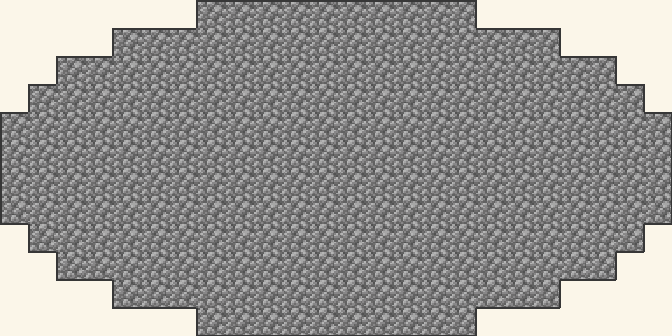
\includegraphics[width=0.45\textwidth]{fig07_2d_ellipse_24x12.png}
\caption{Эллипс $W = 24, H = 12$ в Block Round. Обратите внимание, как клетки вдоль большой оси расставлены реже, чем вдоль малой.}
\label{fig:elipse}
\end{figure}

\begin{enumerate}[leftmargin=1.5em,itemsep=0.15em,topsep=0.3em]
  \item Сменить форму на \acc{Ellipse}. Появятся два \emph{слайдера}: \emph{Width} и \emph{Height}.
  \item Установить $W = 24$, $H = 12$. Посмотреть на удлинённую форму --- рис.~\ref{fig:elipse}.
  \item Обсудить: \emph{«Уравнение, управляющее этой формой, имеет вид $(x/12)^2 + (y/6)^2 = 1$. Почему мы делим $x$ на $12$, а $y$ на $6$?»}
\end{enumerate}

\subsection{Режим 3D, сфера и эллипсоид}

\begin{enumerate}[leftmargin=1.5em,itemsep=0.15em,topsep=0.3em]
  \item Сменить режим на \acc{3D / Sphere}, размер $D = 12$.
  \item Перетаскивать \emph{мышью} для вращения. Появляется сфера, состоящая из вокселей.
  \item Активировать \emph{Info chip}: записать объём («904 блока $=14 \times 64 + 8$»).
  \item Сменить на \acc{Ellipsoid}, $W = 20$, $H = 10$, $D = 12$.
  \item Продемонстрировать \emph{слайдер Cut} на оси \texttt{Y}, 50\,\% (см.\ рис.~\ref{fig:cortes}(a)). Верхняя половина исчезает.
  \item Переключиться на диагональную ось $\swarrow$/$\nearrow$ ($45^\circ$, рис.~\ref{fig:cortes}(c)). Обсудить косой срез.
\end{enumerate}

\subsection{Экспорт в Minecraft}
\begin{enumerate}[leftmargin=1.5em,itemsep=0.15em,topsep=0.3em]
  \item Показать кнопку \emph{скачать} в углу холста: PNG.
  \item Показать кнопку \emph{экспортировать схему}: сохраняет файл \texttt{.schem} в формате Sponge v2.
  \item Если возможно, продемонстрировать импорт в Minecraft Java через мод Litematica. См. Приложение~\ref{ap:litematica}.
\end{enumerate}

% =============================================================================
\newpage
\section{Список упражнений}\label{ap:exerc}

\textbf{Инструкции:} выполнить индивидуально. Можно сверяться с Block Round для подтверждения ответов, \emph{но математическое обоснование обязательно}. Сдать рукописно или в напечатанном виде.

\subsection*{Упражнение 1 --- Уравнение окружности}
\textbf{Условие:} Рассмотрим окружность с центром в начале координат $(0, 0)$ и радиусом $r = 7$. Определите для каждой из следующих точек, находится ли она \emph{внутри}, \emph{снаружи} или \emph{на} окружности. Обоснуйте ответ через уравнение.
\begin{enumerate}[label=\alph*),leftmargin=1.5em,itemsep=0.1em,topsep=0.2em,nosep]
  \item $(3, 4)$ \hfill \emph{ответ:} внутри ($9 + 16 = 25 < 49$).
  \item $(5, 5)$ \hfill \emph{ответ:} \acc{снаружи} ($25 + 25 = 50 > 49$, поскольку $\sqrt{50} \approx 7{,}07$).
  \item $(0, 7)$ \hfill \emph{ответ:} на окружности.
  \item $(-7, 0)$ \hfill \emph{ответ:} на окружности.
\end{enumerate}

\textit{Педагогическое примечание:} пункт (б) --- сознательная ловушка.

\subsection*{Упражнение 2 --- Арифметика стаков и сундуков}
\textbf{Условие:} Рассмотрим сферу $D = 8$ в евклидовом алгоритме, с непрерывным объёмом $V = \tfrac{4}{3}\pi \cdot 4^3 \approx 268{,}1$ и дискретным объёмом $V_{\mathrm{disc}} = 268$.
\begin{enumerate}[label=\alph*),leftmargin=1.5em,itemsep=0.1em,topsep=0.2em,nosep]
  \item Сколько стаков булыжника нужно для её постройки? Ответ в виде $q$ стаков $+$ $r$ блоков.
  \item Сколько обычных сундуков (27 ячеек) понадобится для хранения всех этих стаков?
  \item В режиме выживания, при добыче 1 блока каждые 0{,}5 секунды железной киркой, сколько времени займёт сбор материала?
\end{enumerate}

\emph{Ответ:} (а) $268 = 4 \times 64 + 12$, то есть \acc{4 полных стака $+$ 12 блоков} (5 ячеек в инвентаре). (б) 1 обычного сундука достаточно (из 27 ячеек заняты только 5). (в) $268 \times 0{,}5 = 134$ секунды $\approx$ 2 мин 14 с.

\subsection*{Упражнение 3 --- Сравнение алгоритмов для D=20}
\textbf{Условие:} В Block Round сгенерируйте круг диаметра $D = 20$ в трёх алгоритмах.
\begin{enumerate}[label=\alph*),leftmargin=1.5em,itemsep=0.1em,topsep=0.2em,nosep]
  \item Запишите площадь (число блоков) для каждого алгоритма.
  \item Какой алгоритм минимизирует материал? Какой максимизирует?
  \item Разница в \emph{стаках} между наибольшим и наименьшим? Стоит ли выбирать наименьший ради экономии?
\end{enumerate}

\emph{Ожидаемый ответ:} Евклидов $\approx 316$ блоков (4 стака $+$ 60 экстра), Брезенхэма $\approx 316$, Пороговый $\approx 332$ блока (5 стаков $+$ 12 экстра). Разница: $\approx 1$ стак. В большом проекте (сферы $D \geq 32$) экономия накапливается значительно.

\subsection*{Упражнение 4 --- Объём купола и хранение}
\textbf{Условие:} Рассмотрим сферу $D = 16$, Евклидов алгоритм, срезанную по Y на 50\,\% (классический купол).
\begin{enumerate}[label=\alph*),leftmargin=1.5em,itemsep=0.1em,topsep=0.2em,nosep]
  \item Непрерывный объём полной сферы.
  \item Объём купола (верхняя половина).
  \item Сколько двойных сундуков нужно для хранения всех блоков купола?
  \item Хватит ли остатка на постройку плоского пола $16 \times 16$ блоков под куполом?
\end{enumerate}

\emph{Ответ:}
(а) $V = \tfrac{4}{3}\pi \cdot 8^3 \approx 2\,144{,}66$, $V_{\mathrm{disc}} \approx 2\,145$. (б) $V_{\mathrm{купол}} \approx 1\,095$. (в) $\lceil 1\,095 / 3\,456 \rceil = 1$ двойной сундук. (г) Остаток: $3\,456 - 1\,095 = 2\,361$ блок. Пол $16 \times 16 = 256$ блоков. Остаётся 2\,105 блоков --- хватит и на пол, и на ещё один слой настила.

\subsection*{Упражнение 5 --- Эллипсоид «большой круглый стол»}
\textbf{Условие:} Рассмотрим эллипсоид с $W = 24$, $H = 8$, $D = 24$ (приплюснутая форма «стола»).
\begin{enumerate}[label=\alph*),leftmargin=1.5em,itemsep=0.1em,topsep=0.2em,nosep]
  \item Непрерывный объём.
  \item Дискретный объём, оценённый в Block Round.
  \item Останется или не хватит материала, если куплено 3 двойных сундука дубовых досок?
\end{enumerate}

\emph{Ответ:}
(а) $V = \tfrac{4}{3}\pi \cdot 12 \cdot 4 \cdot 12 \approx 2\,413$.
(б) $V_{\mathrm{disc}} \approx 2\,400$ (варьирует $\pm 10$ по алгоритму).
(в) Купленная вместимость: $3 \times 3\,456 = 10\,368$ блоков. Большой избыток --- $\approx 8\,000$ блоков лишних. \emph{Закуплено чрезмерно.} Идеально --- 1 двойной сундук (избыток $\approx 1\,000$ блоков).

\subsection*{Упражнение 6 --- WorldEdit против Block Round}
\textbf{Условие:} Команда WorldEdit \cmd{//sphere stone 15} использует алгоритм, близкий к 3D-Брезенхэма. Сравните её с выходом Block Round в режиме Брезенхэма при $D = 30$:
\begin{enumerate}[label=\alph*),leftmargin=1.5em,itemsep=0.1em,topsep=0.2em,nosep]
  \item Должны ли они быть идентичны?
  \item Если нет, то почему? Назовите по меньшей мере две причины.
\end{enumerate}

\emph{Ответ:}
(а) \emph{Приблизительно да} --- оба --- 3D-Брезенхэма, но (б) могут различаться по: (i) разным реализациям (Block Round --- на JavaScript, WorldEdit --- на Java); (ii) обработке чётности диаметра (чётный против нечётного); (iii) эмпирической константе \emph{порога} (если один из них внутренне использует Пороговый). Типичная разница: 0--6 блоков при $D = 30$.

\subsection*{Упражнение 7 --- Постройка через октаэдрическую симметрию}
\textbf{Условие:} Спланируйте постройку сферы $D = 16$ с центром в $(0, 72, 0)$ в Minecraft, используя симметрию. Постройте 1 октант (область $+x, +y, +z$, $\approx 268$ блоков) и отразите 7 раз через \cmd{/clone}.
\begin{enumerate}[label=\alph*),leftmargin=1.5em,itemsep=0.1em,topsep=0.2em,nosep]
  \item Напишите 7 команд \cmd{/clone} (используйте \cmd{mode:masked}, чтобы не стирать ландшафт).
  \item Оцените общее время: ручная постройка октанта + команды.
\end{enumerate}

\emph{Ответ:}

\begin{minecraft}[Последовательность команд]
\cmd{/clone 0 72 0 7 79 7 -8 72 0 mode:masked} \quad (отраж.\ $-x$)\\
\cmd{/clone 0 72 0 7 79 7 0 64 0 mode:masked} \quad\quad (отраж.\ $-y$)\\
\cmd{/clone 0 72 0 7 79 7 0 72 -8 mode:masked} \quad (отраж.\ $-z$)\\
\cmd{/clone -8 72 0 -1 79 7 mode:masked} \quad\quad\;\; (октант $-x,-y$)\\
\cmd{/clone 0 64 -8 7 71 -1 mode:masked} \quad\quad\;\; (октант $-y,-z$)\\
\cmd{/clone -8 72 -8 -1 79 -1 mode:masked} \quad\;\; (октант $-x,-z$)\\
\cmd{/clone -8 64 -8 -1 71 -1 mode:masked} \quad\;\; (октант $-x,-y,-z$)
\end{minecraft}

Время: $\sim$\,5 мин (октант вручную в выживании) + $\sim$\,3 с (7 клонов).

\subsection*{Упражнение 8 --- Финальный проект}
\textbf{Условие:} После создания постройки в группе (Задание~\ref{at:53}), ответьте:
\begin{enumerate}[label=(\arabic*),leftmargin=1.7em,itemsep=0.15em,topsep=0.2em,nosep]
  \item Перечислите использованные геометрические фигуры (окружность, эллипс, сфера, эллипсоид) и их параметры (диаметр или полуоси).
  \item Для главной фигуры: какой алгоритм был выбран? Почему? Какой визуальный эффект он производит, недостижимый для двух других?
  \item Были ли 3D-срезы? Если да, опишите математически \emph{один} из них как неравенство.
  \item Сколько стаков/сундуков потребовалось бы для реальной постройки в Minecraft в режиме выживания?
  \item Ваша работа диалогирует с какой-нибудь культурной традицией России (русский авангард, традиционное деревянное зодчество, традиционное жилище коренных народов, шуховские конструкции, русскоязычное Minecraft-сообщество)? Прокомментируйте.
\end{enumerate}

% =============================================================================
\newpage
\section{Адаптация для школ без компьютерного класса}\label{ap:adapt-analog}

Эта адаптация позволяет провести последовательность \emph{полностью на бумаге}, когда доступ к компьютерам затруднён --- частая реальность в школах труднодоступных регионов Заполярья, Сибири, Дальнего Востока, а также в малокомплектных сельских школах. Концептуальная основа остаётся неизменной; меняется только материальный носитель.

\subsection{Замены по урокам}

\begin{center}
\small
\begin{tabularx}{\textwidth}{@{}p{0.13\textwidth}p{0.32\textwidth}X@{}}
\toprule
\textbf{Урок} & \textbf{Оригинальная активность} & \textbf{Аналоговая адаптация} \\
\midrule
1 & Демонстрация Block Round (1.3) & Учитель чертит от руки три варианта окружности $D = 10$ на предварительно подготовленной сетке размером с доску --- по одному на алгоритм. Рис.~\ref{fig:comp-d10} и~\ref{fig:comp-d20} можно распечатать в качестве эталона. \\
\addlinespace[3pt]
2 & Количественное сравнение в ПО (\ref{at:25}) & Раздать листы с тремя окружностями $D = 16$, предварительно нарисованными, и попросить ручной подсчёт клеток. \\
\addlinespace[3pt]
3 & Генерация 3D-сферы (\ref{at:31},~\ref{at:32}) & Раздать листы с \emph{срезами} сферы ($z = 0, 1, 2, \ldots$) на клетчатой бумаге. Ученик собирает ментальную модель сложением. Каждый лист имитирует \emph{слой} блоков Minecraft. \\
\addlinespace[3pt]
4 & Команды Minecraft (\ref{at:42}) & Заменить команды \emph{инструкциями строительства} на русском языке; ученики моделируют выполнение на клетчатой бумаге. \\
\addlinespace[3pt]
5 & Реальная постройка в Minecraft (\ref{at:53}) & Постройка из \emph{ЛЕГО} (если есть), из раскрашенной клетчатой бумаги травянисто-зелёным и коричневым карандашом, или из \emph{бумажных кубиков}, сложенных учениками на уроке труда. \\
\bottomrule
\end{tabularx}
\end{center}

\subsection{Вспомогательные листы}
Для полной аналоговой версии рекомендуется заранее подготовить:
\begin{itemize}[leftmargin=1.3em,itemsep=0.1em,topsep=0.2em,nosep]
  \item 1 лист A3 с сеткой $30 \times 30$, нарисованной линейкой.
  \item 1 комплект на ученика из 5 листов A4 клетчатой бумаги (5\,мм).
  \item 1 лист с тремя сравнительными окружностями, заранее распечатанными: рис.~\ref{fig:comp-d10} и~\ref{fig:comp-d20} этого плана, в A4, служат эталоном.
  \item Для аналогового Урока 5: 8 заранее склеенных бумажных кубиков на группу (представляющих булыжник, дуб, кварц, алмаз).
\end{itemize}

\subsection{Использование местных традиций}
В школах с обучением на родном языке коренных народов России и в местностях с сильной традицией ремёсел (вологодское кружево, гжельская роспись, хохломская роспись, палехская миниатюра, чеченская башенная архитектура, бурятский орнамент, якутская резьба по кости, нанайская вышивка, чукотская резьба по моржовому клыку) Урок~\ref{aula3} может быть \emph{обогащён визитом носителя традиционного знания}: мастеров-ремесленников, плотников, ткачих --- показывающих, как они «растеризуют» круги в своих собственных языках. Это сближение реализует этно\-мате\-ма\-ти\-чес\-кий принцип и Закон «О языках народов Российской Федерации» (1991).

% =============================================================================
\newpage
\section{Технический глоссарий для учителя}\label{ap:glos}

\begin{itemize}[leftmargin=1.4em,itemsep=0.3em,topsep=0.3em]
  \item \acc{Алгоритм} --- конечная и хорошо определённая последовательность инструкций для решения задачи. Три алгоритма Block Round (ср.\ рис.~\ref{fig:comp-d10}) --- разные процедуры для одной задачи.
  \item \acc{Сундук (обычный)} --- контейнер Minecraft на 27 ячеек. Вместимость: $27 \times 64 = 1\,728$ предметов.
  \item \acc{Двойной сундук} --- два соседних сундука, объединённые в контейнер на 54 ячейки. Вместимость: $54 \times 64 = 3\,456$ предметов.
  \item \acc{Блок} --- строительная единица Minecraft. Куб $1\times1\times1$ с шестью текстурированными гранями. На языке математики --- \emph{воксель}.
  \item \acc{Брезенхэма (алгоритм)} --- алгоритм, опубликованный в 1965 году Джеком Брезенхэмом (IBM), изначально для прямой, потом обобщённый другими авторами (Питтвей, Каппел) для эллипса. Главная особенность --- использование \emph{только целых чисел}. См. Задание~\ref{at:23}.
  \item \acc{ФГОС СОО} --- Федеральный государственный образовательный стандарт среднего общего образования. Нормативный документ Российской Федерации для среднего общего образования (10--11 классы).
  \item \acc{Canvas} --- HTML-элемент, предоставляющий пространство 2D или 3D рисунка в браузере.
  \item \acc{\code{/clone}} --- ванильная команда Minecraft, копирующая прямоугольную область в другую позицию. Синтаксис: \cmd{/clone x1 y1 z1 x2 y2 z2 dx dy dz}. Существенна для построек по симметрии.
  \item \acc{ЕГЭ} --- Единый государственный экзамен. Государственный итоговый экзамен в Российской Федерации, проводимый по итогам 11-го класса.
  \item \acc{Неявное уравнение} --- уравнение вида $F(x, y) = 0$. У эллипса: $(x/r_x)^2 + (y/r_y)^2 - 1 = 0$.
  \item \acc{Этноматематика} --- область исследований, основанная бразильцем Убиратаном Д'Амбросио. В русском контексте развивается работами В. Дробышева и др.
  \item \acc{\code{/fill}} --- ванильная команда Minecraft, заполняющая прямоугольную область одним типом блоков. Синтаксис: \cmd{/fill x1 y1 z1 x2 y2 z2 minecraft:stone}.
  \item \acc{МИАН} --- Математический институт имени В. А. Стеклова Российской академии наук (\url{https://www.mathnet.ru/}). Ведущий научно-исследовательский центр чистой математики России в Москве. ПОМИ --- Санкт-Петербургское отделение МИАН.
  \item \acc{ФЗ-152} --- Федеральный закон от 27.07.2006 № 152-ФЗ «О персональных данных».
  \item \acc{Litematica} --- популярный мод для Minecraft Java Edition, импортирующий схемы и показывающий полупрозрачный \emph{призрак} постройки, которую надо реализовать блок за блоком. Бесплатный.
  \item \acc{Minecraft Education Edition} --- образовательная версия Minecraft; в России доступна с ограничениями после 2022 года.
  \item \acc{ВсОШ} --- Всероссийская олимпиада школьников. Крупнейшая олимпиада по математике, информатике, физике и др. в России.
  \item \acc{Pack / Stack} --- стопка до 64 одинаковых блоков в ячейке инвентаря Minecraft.
  \item \acc{Пиксель} --- сокр. от \emph{picture element}. В 2D.
  \item \acc{PWA} --- \emph{Progressive Web App}. Веб-приложение, устанавливаемое и работающее \emph{офлайн}.
  \item \acc{Растеризация} --- процесс преобразования непрерывного геометрического описания в матрицу пикселей (2D) или вокселей (3D).
  \item \acc{Schematica} --- альтернатива Litematica с похожим функционалом.
  \item \acc{Schematic (\texttt{.schem})} --- формат файла, сериализующий область Minecraft (Sponge Schematic v2, gzip + NBT).
  \item \acc{Полуось} --- в эллипсе: расстояние от центра до конца оси.
  \item \acc{\code{//sphere}} --- команда WorldEdit, строящая сферу. Синтаксис: \cmd{//sphere блок радиус}.
  \item \acc{Слот} --- отдельная ячейка инвентаря Minecraft. Полный инвентарь игрока: 36 слотов ($9 \times 4$).
  \item \acc{Воксель} --- сокр. от \emph{volume element}. Обобщение пикселя на 3D. В Minecraft каждый \emph{блок} --- воксель.
  \item \acc{WebGL} --- библиотека программирования 3D-графики для браузеров.
  \item \acc{WorldEdit} --- очень популярный мод Minecraft Java, добавляющий продвинутые команды массовой постройки, включая \cmd{//sphere}, \cmd{//hsphere}, \cmd{//ellipsoid}, \cmd{//cyl}, \cmd{//schem load}.
\end{itemize}

% =============================================================================
\newpage
\section{Руководство: от Block Round к Minecraft через Litematica}\label{ap:litematica}

Это приложение описывает полный поток экспорта из Block Round и импорта в Minecraft Java Edition с использованием мода \emph{Litematica}. Ожидаемое время: 15 минут (первый раз).

\subsection{Предварительные требования}
\begin{itemize}[leftmargin=1.3em,itemsep=0.1em,topsep=0.2em,nosep]
  \item Minecraft Java Edition (покупка в \emph{Mojang Store}; на территории России лицензию можно приобрести через российских реселлеров или альтернативные платёжные сервисы по официальной информации Mojang/Microsoft).
  \item \emph{Fabric Loader} для вашей версии Minecraft (обычно самая свежая: \url{https://fabricmc.net/use/}).
  \item Моды: \emph{Fabric API} и \emph{Litematica} (\url{https://www.curseforge.com/minecraft/mc-mods/litematica}).
  \item Block Round, открытый в браузере, с уже подготовленной фигурой.
\end{itemize}

\subsection{Шаг 1: экспорт из Block Round}
\begin{enumerate}[leftmargin=1.5em,itemsep=0.15em,topsep=0.3em]
  \item В Block Round задайте желаемую фигуру (режим, форма, диаметр, алгоритм, блок, срез). Проверьте объём в \emph{Info chip}.
  \item Нажмите кнопку \emph{Export Schematic} (верхний правый угол холста, вторая иконка). Файл \texttt{.schem} скачается.
\end{enumerate}

\subsection{Шаг 2: установка Litematica}
\begin{enumerate}[leftmargin=1.5em,itemsep=0.15em,topsep=0.3em]
  \item Установите Fabric Loader для вашей версии Minecraft.
  \item Скачайте \emph{Fabric API} и \emph{Litematica} для той же версии Minecraft. Положите оба файла в каталог \texttt{.minecraft/mods/}.
  \item Запустите Minecraft с профилем \emph{fabric-loader-x.y.z-1.20.x}.
\end{enumerate}

\subsection{Шаг 3: импорт схемы}
\begin{enumerate}[leftmargin=1.5em,itemsep=0.15em,topsep=0.3em]
  \item Поместите файл \texttt{.schem} в \texttt{.minecraft/schematics/} (или в папку по умолчанию Litematica, заданную в Настройках мода).
  \item В мире (творческом или выживания) нажмите \texttt{M}, чтобы открыть меню Litematica.
  \item Нажмите \emph{Load Schematic} $\rightarrow$ выберите файл $\rightarrow$ \emph{Load}.
  \item Схема теперь в списке. Нажмите на неё и выберите \emph{Placement}: полупрозрачный «призрак» фигуры появится в мире.
  \item Используйте контролы движения (\texttt{M} $\rightarrow$ \emph{Placements}), чтобы перетащить призрак в нужную позицию. Для плоского ландшафта достаточно поставить нижний угол $(x_1, y_1, z_1)$ на землю.
\end{enumerate}

\subsection{Шаг 4: постройка}
\begin{enumerate}[leftmargin=1.5em,itemsep=0.15em,topsep=0.3em]
  \item В \emph{Creative}: летите над призраком и ставьте каждый блок там, где Litematica показывает; мод подтверждает зелёным правильно расставленные блоки и подсвечивает красным любую ошибку. Постройка сферы $D = 12$ занимает $\approx$\,5 минут.
  \item В \emph{Survival}: то же самое, но материал нужно сначала добыть. Используйте подсчёт стаков/сундуков из Задания~\ref{at:41} для планирования добычи.
  \item Альтернатива: если на сервере стоит WorldEdit, используйте \cmd{//schem load имя-файла} с последующим \cmd{//paste -a} для мгновенной постройки.
\end{enumerate}

\subsection{Шаг 5: проверка}
Litematica подсвечивает красным любой блок, который поставлен неверно (отсутствует, неправильного типа или в неправильной позиции). Используйте сочетание \texttt{Z} для переключения между \emph{видимым} и \emph{невидимым} призраком, сравнивая с реальной постройкой.

\subsection{Решение типичных проблем}
\begin{itemize}[leftmargin=1.3em,itemsep=0.15em,topsep=0.3em,nosep]
  \item \emph{Схема не появляется в списке:} проверьте, что файл находится в нужной папке, и что версия Litematica совместима с версией Minecraft.
  \item \emph{Неправильные/серые блоки:} некоторые блоки в схеме Block Round могут быть недоступны в вашем мире (старая версия Minecraft); откройте схему в текстовом редакторе для проверки имён блоков.
  \item \emph{Призрак висит в воздухе:} настройте позицию через опцию \emph{Rotation/Mirror} в меню Placement. Для сфер это безразлично; для эллипсов отрегулируйте поворот.
\end{itemize}

\vspace{2em}
\begin{center}
\color{muted}\small\sffamily
--- конец плана урока ---
\end{center}

\end{document}
